\documentclass[12pt, openany]{book}
\usepackage{fontspec} % For loading fonts

% This is all the packages and settings and so on.
% It is using custom fonts that needs to be installed on the computer. If they are not present, they have to be added manually.

\usepackage[
    %citestyle=ieee, 
    %bibstyle=ieee,
    style=alphabetic,
    sorting=nty, % Name, title, year
    maxbibnames=99, % Make sure we are printing all authors in the appendix
    backend=biber
    ]{biblatex}

\addbibresource{references.bib}

% Makes the last name first in the bibliography.
% \DeclareNameAlias{author}{last-first}
\DeclareNameAlias{author}{family-given}
    
% Specify the margins. This is 6.25inches in text with which 
% can be used to size figures to the correct size.
\usepackage[a4paper, margin=2.5625cm]{geometry}

\usepackage{eso-pic}					% Packages for layout and graphics 
\usepackage{graphicx}
\usepackage{tikz}
\usetikzlibrary{fadings}
\usepackage{setspace}
\usepackage[hidelinks]{hyperref}		% Clickable links
% \tocloftpagestyle{plain}  
%\usepackage{chngcntr}					% Count figures within chapters
\usepackage{booktabs}					% Table formatting
\usepackage{bookmark}          % Bookmarks in the pdf
\usepackage{fancyhdr}					% Setting the style for header and footer.
\usepackage{tabularx}
\usepackage{multirow}                   % For better tables 
\usepackage{nameref}					% References with names
\usepackage[parfill]{parskip}			% New line instead of indent for sections
\usepackage{tcolorbox}					% Create boxes around content
\tcbset{colback=white,arc=0mm}

\usepackage{amsmath}
\usepackage{mathdots}
\usepackage{yhmath}
\usepackage{siunitx}
\usepackage{array}
\usepackage{gensymb}
\usepackage{amssymb}
\usepackage{mathtools}              % Add text to math arrows.
\usepackage{mathrsfs}

\usepackage{cancel}
\usepackage{color}
\usepackage{multirow}
\usepackage{textcomp}               % Fixing warning for gensyb \perthousand
\usepackage{svg}                    % including svg files
\usepackage{caption}                % For subfigures
\usepackage{subcaption}
\usepackage{sectsty}
\usepackage{tocloft}
\usepackage{etoc} 						% Separate tocs for appendix and the rest  
% GPT4 suggested packages
\makeatletter
\newcount\Etoc@savedtocdepth
\makeatother


\usepackage[printonlyused]{acronym}


%\counterwithin{figure}{section} 
%\counterwithin{table}{section}

% Specifying fonts
%\setmainfont{Georgia} 
%\setsansfont{Arial}
%\newfontfamily\footerfont{Georgia}

\chapterfont{\sffamily\fontsize{17}{17}}
\sectionfont{\sffamily\fontsize{14}{15}}
\subsectionfont{\sffamily\fontsize{13}{15}}
\subsubsectionfont{\sffamily\fontsize{12}{15}}

% Remove the title and make sure that the text is adjusted
% \usepackage{abstract}
% \setlength{\absleftindent}{0mm}
% \renewcommand{\abstractname}{\vspace{-\baselineskip}}
% \renewcommand{\abstractnamefont}{\sffamily\fontsize{14}{15}}
% \renewcommand{\abstracttextfont}{\normalfont\fontsize{12}{13}}

% Renaming and setting style of table of contents
\renewcommand*\contentsname{Contents}
\renewcommand*\cfttoctitlefont{\fontsize{16}{0}\bf\sffamily}
\renewcommand\cftchapfont{\fontsize{14}{0}\bf\sffamily}
\renewcommand\cftchappagefont{\fontsize{13}{0}\bf\sffamily}
\renewcommand\cftsecfont{\fontsize{12}{0}\sffamily}
\renewcommand\cftsecpagefont{\fontsize{12}{0}\sffamily}
\renewcommand\cftsubsecfont{\fontsize{12}{0}\sffamily}
\renewcommand\cftsubsecpagefont{\fontsize{12}{0}\sffamily}

% Styling the header and footer
\fancyhf{}
\fancyhead{}
\fancyfoot{}
\fancyhead[L]{\fontsize{11}{10}\selectfont\leftmark}
\fancyfoot[R]{\thepage}
\setlength{\headheight}{15.5pt}

\fancypagestyle{plain}{
    \fancyhf{}
    \fancyhead{}
    \fancyfoot{}
    \renewcommand{\headrulewidth}{0pt}
    \fancyfoot[R]{\thepage}
}

\pagestyle{fancy}

% Making the command for placing text in random locations
\newcommand\PlaceText[3]{%
\begin{tikzpicture}[remember picture,overlay]
\node[outer sep=0pt,inner sep=0pt,anchor=south west] 
  at ([xshift=#1,yshift=-#2]current page.north west) {#3};
\end{tikzpicture}%
}

% Disable hyphenation
\pretolerance=10000
\tolerance=2000 
\emergencystretch=50pt

% My own stuff
\usepackage{amsthm} % So theoremstyle doesn't print out argument
\newtheorem{theorem}{Theorem}
\theoremstyle{definition}
\newtheorem{definition}{Definition} 
\theoremstyle{remark}
\newtheorem*{remark}{Remark}

\usepackage{tikz-cd} % For diagram 
\usepackage{enumitem} % For bullet enumeration

\usepackage{xcolor}
\newcommand{\mrnote}[1]{\textcolor{red}{#1}}
\newcommand{\mbnote}[1]{\textcolor{blue}{#1}}

\renewcommand{\thefigure}{\arabic{figure}}
\usepackage{relsize} % For big \sigma
\hbadness=10000


% Defining document information
\title{Homomorphic Encryption}
\newcommand{\subtitle}{KTH Thesis Report}
\author{Daniel Sanaee}

\begin{document}
\setstretch{1.4}

% The front page of the document
\pagenumbering{roman}
\makeatletter
\begin{titlepage}

\vspace*{-4.6\baselineskip}
\hspace*{-0.15\textwidth}
\includegraphics[width=0.2\paperwidth]{setup/img/kth-logo.jpg}
\par\vspace*{2.5\baselineskip}

\PlaceText{65mm}{12mm}{\fontsize{12}{0}\sffamily DEGREE PROJECT IN TECHNOLOGY,}
\PlaceText{65mm}{17mm}{\fontsize{12}{0}\sffamily SECOND CYCLE, 30 CREDITS}
\PlaceText{65mm}{22mm}{\fontsize{12}{0}\sffamily\itshape STOCKHOLM, SWEDEN \the\year}

~\\

\makebox[0pt][l]{%
\begin{minipage}[b]{0.25\textwidth}
~\\
\end{minipage}
\begin{minipage}{0.65\textwidth}
\begin{flushleft}
{\fontsize{28}{24}\bf\sffamily\@title\\}
\vspace{1cm}
{\fontsize{19}{17}\bf\sffamily \subtitle\\}
\vspace{1cm} 
{\fontsize{16}{18}\sffamily \@author}\\
\end{flushleft}
\end{minipage}
}


% \hspace*{-3cm}\begin{minipage}[b]{63.5mm}
% ~\\
% \end{minipage}
% \begin{minipage}{0.65\textwidth}
% \begin{flushleft}
% {\fontsize{28}{24}\bf\sffamily\@title\\}
% \vspace{0.5cm}
% {\fontsize{19}{17}\bf\sffamily \subtitle\\}
% \vspace{0.5cm} 
% {\fontsize{16}{0}\sffamily \@author}\\
% \end{flushleft}
% \end{minipage}


\AddToShipoutPictureBG*{%]
    \AtPageLowerLeft{%
        
\includegraphics[width=1.0\paperwidth]{setup/img/kth-footer.png}
    }%
}

\PlaceText{70mm}{280mm}{\color{white}\fontsize{12}{0}\sffamily KTH ROYAL INSTITUTE OF TECHNOLOGY }
\PlaceText{70mm}{285mm}{\color{white}\fontsize{8}{0}\sffamily MATHEMATICS }
\end{titlepage}
\makeatother

\newpage
\newpage
\thispagestyle{plain}
~\\
\vfill
{ \setstretch{1.1}
	\subsection*{Authors}
	Daniel Sanaee <dsanaee@kth.se>\\
	Mathematics\\
	KTH Royal Institute of Technology
	
	\subsection*{Place for Project}
	Stockholm, Sweden
	
	\subsection*{Examiner and supervisor}
	Johan Håstad\\
	KTH Royal Institute of Technology
	
	~
}

\newpage
\thispagestyle{plain}
%%%%%%%%%%%%%%%%%%%%%%%%%%%%%%%%%%%%
%%  The English abstract          %%
%%%%%%%%%%%%%%%%%%%%%%%%%%%%%%%%%%%%
\chapter*{Abstract}
%%%%%%%%%%%%%%%%%%%%%%%%%%%%%%%%%%%%

\vspace{2cm}
Write an abstract. Introduce the subject area for the project and describe the problems that are solved and described in the thesis. Present how the problems have been solved, methods used and present results for the project. Use probably one sentence for each chapter in the final report.

The presentation of the results should be the main part of the abstract. Use about ½ A4-page.
English abstract




\subsection*{Keywords}
Template, Thesis, Keywords ...





\newpage
\thispagestyle{plain}
%%%%%%%%%%%%%%%%%%%%%%%%%%%%%%%%%%%%
%%	 The Swedish abstract         %%
%%%%%%%%%%%%%%%%%%%%%%%%%%%%%%%%%%%%
\chapter*{Abstract}
%%%%%%%%%%%%%%%%%%%%%%%%%%%%%%%%%%%%
Svenskt abstract
\begin{comment}
Svensk version av abstract – samma titel på svenska som på engelska.

Skriv samma abstract på svenska. Introducera ämnet för projektet och beskriv problemen som löses i materialet. Presentera 
\end{comment}
\subsection*{Nyckelord}
Kandidat examensarbete, ...


\newpage
\thispagestyle{plain}
\chapter*{Acknowledgements}
Write a short acknowledgements. Don't forget to give some credit to the examiner and supervisor.

\newpage

\chapter*{Acronyms}
\begin{comment}
\begin{acronym}[RDBMS]
\acro{ACID}{atomicity, consistency, isolation, and durability}
\acro{CAP}{Consistency, Availability, Partition-tolerant}
\acro{CDF}{Cumulative Distribution Function}
\acro{CPU}{Central Processing Unit}
\end{acronym}
\end{comment}




\newpage

\etocdepthtag.toc{mtchapter}
\etocsettagdepth{mtchapter}{subsection}
\etocsettagdepth{mtappendix}{none}
\thispagestyle{plain}
\tableofcontents

\newpage




\pagenumbering{arabic}

\chapter{Introduction}

Cloud computing is more important

What is homomorphic encryption?
Server calculates on encrypted data and client has the secret key
Applications to real world

Applications: includes machine learning, data storage of sensitive data (medical records, financial records, etc.), GPS, genomic analysis 

\chapter{Computation theory}
 In this section, it is assumed that the reader has prior knowledge of deterministic- and probabilistic Turing machines as a model of computation (an excellent introduction can be found in \cite{Gol01}). We introduce an alternative model of computation based on sets of circuits for the purpose of protection against stronger adversaries. We include the basics needed to understand cryptography and homomorphic encryption in particular. 

\section{Digital logic}

\begin{definition}[Circuit]
For $n, m \in \mathbb{N}$ and any field $(\mathbb{F},+,\times)$, an arithmetic circuit is a vector-valued polynomial function $C \colon \mathbb{F}^{n} \to \mathbb{F}^m$. 
\end{definition}

A circuit $C$ is represented by a finite directed acyclic graph with $n$ source nodes (the $n$ inputs) and $m$ sink nodes (the $m$ outputs). The internal nodes of the circuit are called \emph{gates} and is stacked in layers. For more details about the structure of a circuit, see \cite{goldreich_2008} or \cite{MF21}. The number of nodes in $C$ is called its \emph{size} and is denoted $|C|$. The longest path in $C$ is called its \emph{depth}.
A circuit is called \emph{Boolean} when the field is $\mathbb{F}_2$ and each gate takes at most 2 inputs. Boolean circuits and arithmetic circuits are equivalent in the sense that the set of functions that can be computed by an arithmetic circuit is equal to the set of functions that can be computed by a Boolean circuit.\footnote{A Boolean circuit is an arithmetic circuit. Conversely, any arithmetic circuit can be simulated by representing the inputs and outputs as a bitstring and utilizing that XOR and AND is a complete set of gates.} If the input is a string of bits, we assume the circuit is Boolean.

We consider circuits as algorithms and use them as an alternative approach to the traditional Turing machine model of computation.\footnote{The reason for this alternative model is to assume adversaries are computationally "stronger". See Theorem \ref{thm:compl-class}.} Notice that any given circuit, $C$, can only compute on inputs of the same length whereas a Turing machine $M$ takes inputs of any size $n$. However, a circuit always halts on a given input whereas a Turing machine may not. For the purpose of our discussion relating to cryptography, we assume every Turing machines halts unless otherwise stated. To allow circuits to handle arbitrary length inputs we consider families of circuits.  

\begin{definition}[Circuit family \cite{MF21}]
A circuit family $C = \{C_n\}_{n \in \mathbb{N}}$ is an indexed set of circuits $C_n \colon \mathbb{F}^{n + r} \to \mathbb{F}^m$ where $r,m = \operatorname{poly}(n)$.
\end{definition}

For any input $x$ with length $n$, $C(x) \stackrel{\mathrm{def}}{=} C_n(x)$. For each circuit $C_n \in C$, $r$ represents the random coins used. If $r = 0$ for all $n$ then $C$ is a deterministic circuit family. A circuit family is said to have polynomial-size if there exists a polynomial $p$ such that $|C_n| < p(n)$ for all $n$. 

\section{Complexity classes}\label{subsec:Complexity classes}
\begin{definition}[Complexity Class $\operatorname{P}$]
$\operatorname{P}$ is the set of languages $\mathscr{L}$ such that there exists a deterministic polynomial-time Turing machine $M$ satisfying $M(x) = 1 \iff x \in \mathscr{L}$ 
\end{definition}
\begin{definition}[Complexity Class $\operatorname{BPP}$]
$\operatorname{BPP}$ is the set of languages $\mathscr{L}$ such that there exists a probabilistic polynomial-time (PPT) Turing machine $M$ satisfying
\begin{align*}
& \operatorname{Pr}[M(x)=1] \geq 2/3 \text{ if $x \in L$}
\\
& \operatorname{Pr}[M(x)=1] \leq 1/3 \text{ if $x \notin L$}
\end{align*}
\end{definition}
\begin{definition}[Complexity Class $\operatorname{P/poly}$]
$\operatorname{P/poly}$ is the set of languages $\mathscr{L}$ such that there exists a polynomial-size circuit family $C$ satisfying $C(x) = 1 \iff x \in \mathscr{L}$ 
\end{definition}
Informally speaking, circuit families is a stronger model of computation than the PPT Turing machine model in the sense that if there exists a PPT Turing machine for deciding a problem, then there also exists a circuit family that can decide the same problem. The formal statement is as follows: 
\begin{theorem}
    \label{thm:compl-class}
    $\operatorname{P} \subseteq \operatorname{BPP} \subsetneq \operatorname{P/poly}$
\end{theorem}
The first inclusion follows from the fact that if there exists a deterministic Turing machine that decides a language, then that same machine can be seen as a PPT machine that ignores a given input sequence of coin tosses. For the second inclusion, consider a language $\mathscr{L} \in \operatorname{BPP}$ and a corresponding PPT machine $M$ for $\mathscr{L}$. Then, for any given input $x_n$ with length $n$, at least $2/3$ of the set of all possible coin toss sequences are good (good $r$ means $M(x_n;r) = 1 \iff x_n \in \mathscr{L}$). This means that there exists at least 1 sequence of coin tosses that yields the correct result for $2/3$ of the possible inputs of length $n$. Consider machine $M'$ that on input $x_n$ runs $M(x_n)$ many (still $\operatorname{poly}(n)$) times and outputs the majority result. Then, the error probability vanishes exponentially, meaning there are exponentially few coin toss sequences that are bad for $M'$ (see \cite{Arora,Gol01} for more detail). Therefore there exist a coin toss sequence, $r_n$, that yields the correct result for all inputs of length $n$. Consider circuit $C_n \colon \{0,1\}^{n+|r_n|} \to \{0,1\}$ with $r_n$ hardcoded as inputs where $C_n$ simulates $M'$ using $r_n$, i.e., $C_n(x_n) = M'(x;r)$. Therefore $C_n(x) = 1 \iff x \in \mathscr{L}$ and $C$ decides $\mathscr{L}$.

Interestingly the first inclusion is speculated to be set equivalence \cite[pp. 126]{Arora}, meaning that a deterministic machine could decide the same languages as a probabilistic one. The second inclusion is proper since every unary language is in $\operatorname{P/poly}$ whereas undecidable ones are not in $\operatorname{BPP}$ (see \cite[pp. 110]{Arora} for details). In this sense, circuit families are a stronger model of computation than PPT Turing machines. We capture this notion with uniformity. 

\begin{definition}[Uniform circuit family]
A circuit family $\{C_n\}_{n \in \mathbb{N}}$ is uniform if there exists a polynomial-time Turing machine $M$ such that $M(1^n)$ outputs the description of $C_n$ for all $n\in \mathbb{N}$.
\end{definition}

A uniform circuit family is polynomial size. The converse is not necessarily true. A family that is not uniform is said to be a non-uniform circuit family. Note that Turing machines are at least as strong as uniform circuit families. More formally, if a uniform circuit family decides $\mathscr{L}$ then there exists a polynomial-time Turing machine that decides $\mathscr{L}$.\footnote{The converse is also true, meaning deterministic polynomial-time Turing machines are exactly as powerful as uniform circuit families. See \cite[pp. 111]{Arora} for details} Simply construct the polynomial-time Turing machine that given any input $x \in \mathscr{L}$, first generates a description of $C_{|x|}$ and then simulates $C_{|x|}(x)$. In other words, the non-uniform circuit families are stronger than the polynomial-time Turing machines.

\chapter{Probability Theory}

Homomorphic encryption schemes are based on noise. As we will see in Subsection \ref{subsec:LWE}, noise can be sampled from discrete spaces in accordance with a distribution. Since distributions are central in cryptography, it is important they are understood. A distribution is a probability measure on a measurable space $(S, \mathcal{S})$. Typically, probability distributions are associated with random variables; however, in the absence of random variables, distributions are understood as a specified measure function on the given measurable space (See \cite[pp. 83]{kallenberg-probability}).
\begin{definition}[Discrete distribution measure of a random variable]
Consider a probability space $(\Omega, \mathcal{F}, \operatorname{Pr})$ and a discrete measurable space $(S,\mathcal{S})$. Let $X \colon \Omega \mapsto S$ be a random variable. The discrete distribution measure of $X$, or simply \emph{distribution} of $X$, $\chi$ is defined as follows
\begin{equation*}
\begin{aligned}
    \chi \colon \mathcal{S} &\to [0,1]\\
    \{x\} &\mapsto \operatorname{Pr}[X = x]
\end{aligned}
\end{equation*}
We say that $\chi$ is the distribution or \emph{law} of $X$, denoted $\mathcal{L}(X)$. 
\end{definition}
\begin{remark}
    Since $\chi$ is a measure on a discrete space, the description of the singletons are sufficient. More explicitly, $\chi(A) = \sum_{x \in A} \operatorname{Pr}[X = x]$ for $A \in \mathcal{S}$
\end{remark}
A distribution measure for a random variable is a probability measure on the sample space $(S,\mathcal{S})$, as opposed to on the outcome space $(\Omega, \mathcal{F})$. For a given probability space, any random variable $X$ defined on it has a distribution associated with it. We write $x \leftarrow X$ or $x \leftarrow \chi$ for sampling the outcome $x$ from $X$ assuming $\chi$ is its distribution. When $X$ is a space we mean that $x$ is uniformly sampled from $X$.

\begin{definition}[Ensembles] \label{def:prob-ensemble}
    Let $I$ be a countable index set. A \emph{probability ensemble} indexed by $I$ (or just ensemble) is a sequence of random variables $(X_i)_{i \in I}$. A \emph{distribution ensemble} indexed by $I$ is a sequence of distributions $(\chi_i)_{i \in I}$
\end{definition}
In this paper we will exclusively use $\mathbb{N}$ as the index set.
For example, the encryption function is a random variable (PPT algorithm), meaning that a single message $m$ corresponds to many valid ciphertexts. By varying the security parameter of the scheme we construct the probability ensemble $\{Enc(pk,m)\}_{pk \in \mathbb{N}}$
\begin{definition}[Statistical distance] \label{def:statistical-distance}
    Let $S_n$ be finite set for all $n \in \mathbb{N}$ and let $X = (X_n \colon \Omega_n \to S_n)_{n \in \mathbb{N}}$, $Y = (Y_n \colon \Omega_n \to S_n)_{n \in \mathbb{N}}$ be two ensembles. The \emph{statistical distance} is defined as
    \begin{equation*}
        \Delta_{X,Y}(n) \stackrel{\mathrm{def}}{=} \frac{1}{2} \sum_{\alpha \in S_n} |\operatorname{Pr}[X_n = \alpha] - \operatorname{Pr}[Y_n = \alpha]|.
    \end{equation*}
    Let $\chi = \{\chi_n\}_{n \in \mathbb{N}}$, $\psi = \{\psi_n\}_{n \in \mathbb{N}}$ be two discrete distribution ensembles on the same measurable spaces $\{(S_n, \mathcal{S}_n)\}_{n \in \mathbb{N}}$. The statistical distance is defined as
    \begin{equation*}
    \begin{aligned}
        \Delta_{\chi, \psi}(n) \stackrel{\mathrm{def}}{=} \frac{1}{2} \sum_{\alpha \in S_n} |\chi_n(\{\alpha\}) - \psi_n(\{\alpha\})|
    \end{aligned}
    \end{equation*}
\end{definition}
\begin{remark}
    This definition for distribution ensembles assumes every singleton is measurable. A more general definition is $\Delta(\chi, \psi) \stackrel{\mathrm{def}}{=} \sup _{A \in \mathcal{S}}|\chi(A)-\psi(A)|$ 
\end{remark}

\begin{definition}[Negligible function]
    Let $f \colon \mathbb{N} \to [0,1]$. $f$ is negligible if for all positive polynomials $p(\cdot)$, there exists an $N$ such that for all $n>N$, $f(n) < \frac{1}{p(n)}$. We say $f = \operatorname{negl}(n)$.
\end{definition}
\begin{definition}[Perfectly indistinguishable] \label{def:perfectly-indistinguishable}
    Two ensembles (probability or distribution) $X$ and $Y$ are \emph{perfectly indistinguishable} if $\Delta_{X,Y}(n) = 0$ for all $n$.
\end{definition}
\begin{definition}[Statistically indistinguishable] \label{def:statistically-indistinguishable}
    Two ensembles (probability or distribution) $X$ and $Y$ are \emph{statistically indistinguishable} if $\Delta_{X,Y}(n) = \operatorname{negl}(n)$.
\end{definition}
 A desirable property of encryption schemes is to make it unfeasible for adversaries to distinguish encryptions. For two random variables (or distributions) $X$ and $Y$, we want every adversary $C$ to not be able to distinguish samples from $X$ and $Y$. More precisely, an adversary tasked with identifying whether given samples are from $X$ ($C$ outputs 0) or from $Y$ ($C$ outputs 1) should have roughly the same probability of success irrespective of which the samples are generated from. The formal definition is as follows:
\begin{definition}[Computationally indistinguishable \cite{Gol01}] \label{def:computationally-indistinguishable}
    Two ensembles (or distribution ensembles) $X$ and $Y$ are computationally indistinguishable if, for every polynomial-size circuit family $C = \{C_n\}_{n \in \mathbb{N}}$, $$\operatorname{Adv}_{X,Y}(n) \stackrel{\mathrm{def}}{=} |\operatorname{Pr}[C(X_n) = 1] - \operatorname{Pr}[C(Y_n) = 1]| = \operatorname{negl}(n).$$
\end{definition}
$C(X_n), C(Y_n)$ means that the adversary has access to random oracle returning a sample from $X_n$ and $Y_n$ respectively. The point is that, for every adversary $C$ guessing the samples are from one of the random variables or distributions (1 in this case represents from $Y_n$), the probability of being correct is, up to negligible error, equal to the probability of being incorrect. For example, an adversary always guessing 1 has 100\% probability of being incorrect when given samples from $X_n$ and 100\% probability of being correct when given samples from $Y_n$. The intuition is that the sample does not make a noticable difference on the guess and that the advantage in distinguishing samples goes to zero fast (faster than the inverse of all polynomials).

Perfect distinguishability implies statistical indistinguishability as 0 is negligible. Statistical indistinguishability implies computational indistinguishability. To see why, assume $\Delta_{X,Y}(n) = \operatorname{negl}(n)$ and consider any circuit family $C$. Since $X_n$ and $Y_n$ are defined on the same space we have
\begin{equation*}
\begin{aligned}
    \operatorname{Adv}_{X,Y}(n) &= |\operatorname{Pr}[C(X_n) = 1] - \operatorname{Pr}[C(Y_n) = 1]|\\
        &\leq \sum_{\alpha \in S_n} | \operatorname{Pr}[C(X_n = \alpha) = 1 \; | \; X_n = \alpha]\operatorname{Pr}[X_n = \alpha] \\
        &\phantom{=} \qquad - \operatorname{Pr}[C(Y_n = \alpha) = 1 \; | \; Y_n = \alpha]\operatorname{Pr}[Y_n = \alpha] | \\
        &\leq \sum_{\alpha \in S_n} | \operatorname{Pr}[X_n = \alpha] - \operatorname{Pr}[Y_n = \alpha]| = 2\Delta_{X,Y}(n) = \operatorname{negl}(n)
\end{aligned}
\end{equation*}
where the first inequality is due to the triangle inequality and the second is due to conditional probability being upper bounded by 1. Intuitively, there does not exist enough distinguishable outcomes to distinguish the ensembles even if there exists an adversary that always correctly recognize an outcome from $X$ and $Y$ respectively.
\subsection*{Distributions for noise in HE}
To add discrete noise to ciphertexts, it is typical to use the discretized Gaussian distribution introduced by Micciancio and Regev \cite{disc-gauss}. Since this distribution is used so frequently, we give a brief presentation of it here. A continuous Gaussian distribution in $\mathbb{R}^n$ centered at $\vec{c}$ where each coordinate is independently sampled from normal distirbution with standard deviation $\sigma$, then the multivariate Gaussian distribution is simplified to $\rho_{\vec{c}}(\vec{x}; \sigma)=\frac{1}{\left(2 \pi \sigma^2\right)^{n / 2}} \exp \left(-\frac{1}{2 \sigma^2} \| \vec{x}-\vec{c} \| ^2\right)$. By introducing the scale factor $s \stackrel{\mathrm{def}}{=} \sqrt{2\pi}\sigma$ we get $\rho_{s, \vec{c}}(\vec{x})=\frac{1}{s^n} \exp \left(-\frac{\pi}{s^2} \| \vec{x}-\vec{c} \| ^2\right)$.
The goal is to discretize the gaussian over lattices, see Section \ref{sec:lattices}, by restricting the domain to lattice points. For a given lattice $L \subset \mathbb{R}^n$ we define the normalization constant $\rho_{s, \vec{c}}(L) \stackrel{\mathrm{def}}{=} \sum_{\vec{x} \in L} \rho_{s, \vec{c}}(\vec{x})$.
\begin{definition}[Discrete Gaussian distribution]\label{Disc-Gauss}
    Let $L \subset \mathbb{R}^n$ be a lattice. Then the discrete gaussian distribution is defined as
    \begin{equation*}
        \forall \vec{x} \in L \colon \quad \textrm{D}_{L, s, \vec{c}}(\vec{x}) \stackrel{\mathrm{def}}{=} \frac{\rho_{s, \vec{c}}(\vec{x})}{\rho_{s, \vec{c}}(L)}.
    \end{equation*}            
\end{definition}
\begin{definition}[$\beta$-bounded distribution]
    Let $\chi = \{\chi_n\}_{n\in \mathbb{N}}$ be a distribution ensemble over the integers. $\chi$ is $\beta$-bounded if $x \leftarrow \chi_n \implies |x| < \beta$
\end{definition}
\begin{remark}
    It is also possible (and common) to define a $\beta$-bounded distribution such that $x \geq \beta$ with negligible probability.
\end{remark}
\begin{figure}
    \centering
    \hypertarget{fig:discrete-gauss}{}
    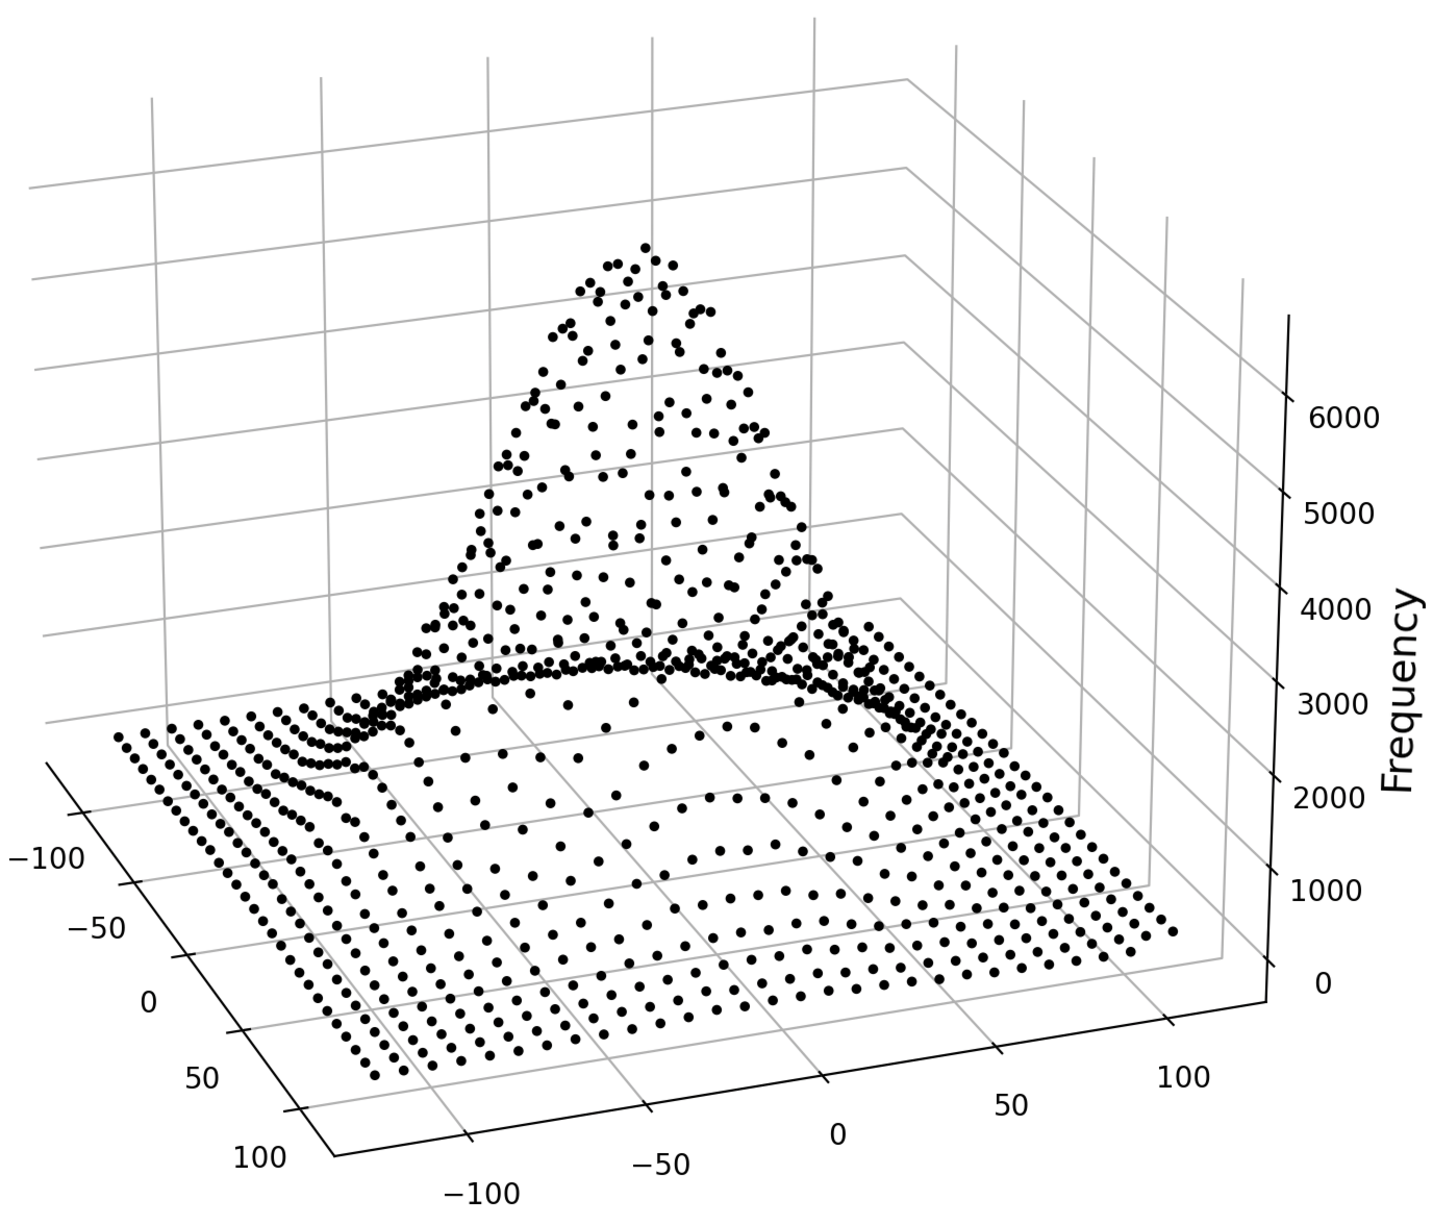
\includegraphics[width=0.65\textwidth]{figures/D-G-2d-a_is_100-n_1000000.pdf}
    \caption*{\textbf{Figure 1}: Discrete Gaussian distribution $\textrm{D}_{\mathbb{Z}^2, 100, \vec{0}}$ with 1 million samples. Every point has integer coordinates. See code in Appendix \ref{app:code}.}
\end{figure}

\chapter{Cryptographic primitives}
In the following definitions we let the message space be denoted $\mathcal{X}$, the ciphertext space be denoted $\mathcal{Y}$, and the key space be denoted $\mathcal{K} = \mathcal{K}_{pk} \times \mathcal{K}_{sk}$.
\begin{definition}[Encryption scheme]
A correct asymmetric \emph{encryption scheme} $\mathcal{E} = (\text{KeyGen, Enc, Dec})$ is a triple of algorithms satisfying the following:
\begin{enumerate}[label={$\bullet$}]
    \item KeyGen $\colon \{1\}^* \to \mathcal{K}$ is PPT given by $1^{\lambda} \mapsto (pk,sk)$.
    \item Enc $\colon \mathcal{K}_{pk} \times \mathcal{X} \to \mathcal{Y}$ is PPT given by $(pk,m) \mapsto c$.
    \item Dec $\colon \mathcal{K}_{sk} \times \mathcal{Y} \to \mathcal{X}$ is deterministic and satisfies $(pk, sk) \leftarrow \operatorname{KeyGen}(1^{\lambda}) \implies \operatorname{Dec}(sk, \operatorname{Enc}(pk,m)) = m$.
\end{enumerate}
\end{definition}
\begin{remark}
This paper is only concerned with encryption schemes where decryption always works (correct) and where more than one key is used (asymmetric). Thus, every encryption scheme is assumed to be a correct asymmetric encryption scheme. Furthermore, the decryption algorithm can be considered a PPT algorithm that with probability 1 outputs the correct message for the correct secret key. In other words, the algorithm ignores the input coin toss sequence.
\end{remark}
In this paper, we consider homomorphic encryption (HE) schemes. These schemes include a fourth algorithm, Eval, called the evaluation algorithm which is used by the server calculating on encrypted data.
\begin{definition}[$\mathcal{C}$-homomorphic encryption scheme]
    \label{def:HE-scheme}
An encryption scheme $\mathcal{E}$ is a \emph{$\mathcal{C}$-homomorphic encryption scheme} for the set of circuits $\mathcal{C}$ if there exists an extra algorithm Eval such that for any $C \in \mathcal{C}$ taking $t$ inputs the following condition holds:
\begin{enumerate}[label={$\bullet$}]
    \item  Eval$ \colon  \mathcal{K}_{pk} \times \mathcal{C} \times \mathcal{Y}^* \to \mathcal{Y}$ is PPT and satisfies $(pk,sk) \leftarrow \operatorname{KeyGen}(1^{\lambda}) \implies \operatorname{Dec}(sk, \operatorname{Eval}(pk, C, \left\langle \operatorname{Enc}(pk, m_1), \dots , \operatorname{Enc}(pk, m_t) \right\rangle)) = C(m_1, \ldots, m_t)$
\end{enumerate}
We say $\mathcal{E}$ can evaluate all circuits in $\mathcal{C}$ and is $\mathcal{C}$-homomorphic.
\end{definition}
The evaluation algorithm runs the ciphertexts through the permissible circuit while also satisfying the requirement that decrypting the resulting ciphertext yields the same result as the plaintexts running through the circuit. To its disposal, the evaluation algorithm is given the public key. The ciphertexts returned by the Eval algorithm are called \emph{evaluated ciphertexts} (suggesting the circuit has evaluated the ciphertexts) and those returned by the encryption algorithm are called \emph{fresh ciphertexts}. Remark that correctness is only guaranteed if the Eval algorithm is given fresh ciphertexts. If the circuit corresponds to the computable function $f$ acting on a vector $c$ of ciphertexts, we denote the evaluated ciphertexts $c_f$ (i.e., $c_f \stackrel{\mathrm{def}}{=} \operatorname{Eval}(pk, f, c)$). Similarly, for the vector $m$ of plaintexts, we denote the evaluated plaintexts $m_f$ (i.e., $m_f \stackrel{\mathrm{def}}{=} f(m)$). Thus, the condition for the Eval algorithm can be written $(pk,sk) \leftarrow \operatorname{KeyGen}(1^{\lambda}) \implies \operatorname{Dec}(sk, c_f) = m_f$.
\begin{figure}
    \[
\begin{tikzcd}[row sep=2cm, column sep=5cm]
\mathcal{Y}^t \arrow{r}{\text{Eval}(pk,C,\left\langle c_1, \dots, c_t \right\rangle) \; = \; c_f} \arrow{d}[swap]{\text{Dec}(sk, \left \langle c_1, \dots, c_t \right\rangle)} & \mathcal{Y} \arrow{d}{\text{Dec}(sk, c_f)} \\
\mathcal{X}^t \arrow{r}[swap]{C(m_1, \dots, m_t)} & \mathcal{X}
\end{tikzcd}
\]

    \caption*{\textbf{Figure 2}: The decryption homomorphism. The path through $\mathcal{Y}$ represents computing before decrypting. The path through $\mathcal{X}^t$ represents decrypting before computing.\label{fig:homomorphism}}
\end{figure}
In a homomorphic encryption scheme that supports one addition and multiplication of fresh ciphertexts, the decryption function is a ring homomorphism. Consider a valid key pair $(sk,pk)$ which are, for notational simplicity, hard-wired into the decryption and evaluate functions respectively, plaintext ciphertext pairs $(m_1,c_1 = \operatorname{Enc}_{pk}(m_1))$, $(m_2, c_2 = \operatorname{Enc}_{pk}(m_2))$ and circuits $C_+(m_1,m_2) \stackrel{\mathrm{def}}{=} m_1 + m_2$ and $C_{\times}(m_1,m_2) \stackrel{\mathrm{def}}{=} m_1 \times m_2$ that can be evaluated by the scheme. 
\begin{equation*}
\begin{aligned}
\operatorname{Dec}_{sk}(c_1 + c_2) &= \operatorname{Dec}_{sk}(\operatorname{Eval}_{pk}(C_+,\left\langle c_1,c_2 \right \rangle) = C_+(m_1,m_2) = m_1 + m_2 \\
    & = \operatorname{Dec}_{sk}(c_1) + \operatorname{Dec}_{sk}(c_2)\\
\operatorname{Dec}_{sk}(c_1 \times c_2) &= \operatorname{Dec}_{sk}(\operatorname{Eval}_{pk}(C_{\times},\left\langle c_1,c_2 \right \rangle) = C_{\times}(m_1,m_2) = m_1 \times m_2 \\
    & = \operatorname{Dec}_{sk}(c_1) \times \operatorname{Dec}_{sk}(c_2)
\end{aligned}
\end{equation*}
The main idea behind a homomorphic encryption scheme is to give a server encrypted data so that it can compute on that data and return the answer in encrypted form. However, the definition provided allows for trivial homomorphic encryption schemes where the server does nothing. More specifically, consider any set of circuits $\mathcal{C}$ and let $\operatorname{Eval}(pk, C,\left\langle c_1, \dots ,c_t \right\rangle) = (C, \left\langle c_1, \dots, c_t \right \rangle)$. Eval takes a description of a circuit and a tuple of ciphertexts, one for each input wire of the circuit, and simply outputs the description of the circuit together with the given tuple. Clearly, Eval runs in polynomial time. Consider a decryption algorithm that, if given an input of this form, first decrypts the $t$ ciphertexts and then computes $m_f$ using $C$. To ensure that the server actually processes the given inputs we introduce compactness.

\begin{definition}[Compactness]
A $\mathcal{C}$-homomorphic encryption scheme is compact if there exists a polynomial $p(\lambda)$ such that for all $(pk,sk) \leftarrow \operatorname{KeyGen}(1^{\lambda})$, for every $C \in \mathcal{C}$ taking any number $t$ inputs and any $c \in \mathcal{Y}^t$, the size of the output $\operatorname{Eval}(pk, C, \left\langle c_1, \dots, c_t \right\rangle)$ is less than $p(\lambda)$. We say that the scheme compactly evaluates $\mathcal{C}$.
\end{definition}

For a compact $\mathcal{C}$-homomorphic encryption scheme, the size of the output is independent of the circuit function used. In particular, the previous, trivial homomorphic encryption scheme where $\operatorname{Eval}(pk, C,\left\langle c_1, \dots ,c_t \right\rangle) = (C, \left\langle c_1, \dots, c_t \right \rangle)$ is not compact for any set of circuits with unbounded circuit size, which includes circuit families with circuits that do not ignore all except for constantly many inputs, meaning essentially every application of a HE scheme.

\begin{definition}[Fully Homomorphic Encryption (pure FHE)]
Let $\mathcal{C}$ be the class of all circuits. An encryption scheme $\mathcal{E}$ is a fully homomorphic encryption (pure FHE) scheme if it is $\mathcal{C}$-homomorphic and compactly evaluates $\mathcal{C}$.
\end{definition}

For a scheme to be fully homomorphic it is required that it can evaluate circuits of arbitrary size. Many times it suffices to consider only circuits of a beforehand specified depth, $L$, as any deeper circuits are irrelevant to the application. The following definition capture schemes that can evaluate any set of circuits with depths bounded by the client.   

\begin{definition}[Leveled fully homomorphic encryption (leveled FHE)]
An encryption scheme $\mathcal{E}$ with the KeyGen algorithm modified is a leveled fully homomorphic encryption scheme if it satisfies the following:
\begin{enumerate}[label={$\bullet$}]
    \item KeyGen $\colon \{1\}^* \times \{1\}^* \to \mathcal{K}$ is PPT given by $(1^{\lambda},1^L) \mapsto (pk,sk)$.
    \item Let $\mathcal{C}_L$ be the set of circuits with depth less than or equal to $L$. Then $\mathcal{E}$ is $\mathcal{C}_L$-homomorphic.
    \item $\mathcal{E}$ compactly evaluates the set of all circuits. 
\end{enumerate}
\end{definition}
\begin{remark}
    Notice that the length of the evaluated ciphertexts in a leveled FHE scheme is independent of the depth.
\end{remark}
For any specified circuit $C$, a leveled FHE scheme can evaluate it by choosing sufficiently large depth parameter, $L$. For a pure FHE scheme, the circuit does not need to be specified. A pure FHE scheme can dynamically compute any circuit whereas the leveled FHE scheme requires the circuit chosen a priori.

\section{Security definitions}

In this paper, semantic security refers to security against chosen-plaintext attack (CPA). The definition relates to the following game where the challenger possess the secret key and the player is the adversary trying to break the scheme. Consider encryption scheme $(\text{KeyGen, Enc, Dec, Eval})$ and polynomial-size Boolean circuit family $C = \{C_n\}_{n\in \mathbb{N}}$. The CPA game is defined with the Boolean function $\operatorname{CPA}_{C}(\lambda)$ as follows:
\begin{enumerate}
  \item \textbf{Setup}: Challenger samples $pk \leftarrow \operatorname{KeyGen}$ and sends it to player.
  \item \textbf{Choose}: Player $C$ selects two distinct plaintext messages $(m_0, m_1) \leftarrow C(pk)$ of the same length, and sends them to the challenger.
  \item \textbf{Encrypt}: The challenger randomly picks a bit $b \in \{0, 1\}$ and encrypts the message $m_b$. The encrypted message $c \stackrel{\mathrm{def}}{=} \operatorname{Enc}(pk, m_b)$, called challenge ciphertext, is sent to the player.
  \item \textbf{Guess}: Player $C$ output guess $b' \in \{0,1\}$.
  \item \textbf{Win}: $\operatorname{CPA}_{C}(\lambda) = 
  \begin{cases}
  1 & \text{if } b = b'\\
  0 & \text{if } b \neq b'.
  \end{cases}$
\end{enumerate}

If $\operatorname{CPA}_{C}(\lambda) = 1$ then the adversary $C$ guessed correctly which of their two chosen messages was encrypted, based only on observing the ciphertext. Notice that the game requires the player to choose messages of equal length in the 'choose' phase since the ciphertext length always leaks information about the length of the message, namely an upper bound on the message length.
\begin{definition}[Semantic security (CPA)]
    An encryption scheme is semantically secure if, for all polynomial-size Boolean circuit families $C$, $$| \operatorname{Pr}[\operatorname{CPA}_{C}(\lambda)] - \frac{1}{2} | = \operatorname{negl}(\lambda).$$
\end{definition}
Semantic security means that there exists no algorithm in $\operatorname{P/poly}$ that can do more than negligibly better than guessing randomly in determining the message. Semantic security is equivalent to indistinguishability of encryptions (see \cite{Gol04} for proof).
\begin{definition}[Indistinguishability of encryptions]
    An encryption scheme has indistinguishable encryptions if for any key $(pk,sk) \leftarrow \operatorname{KeyGen}(1^{\lambda})$ and any two distinct messages $m_1, m_2$ of equal length, the ensembles $\{\operatorname{Enc}(pk,m_1)\}_{\lambda \in \mathbb{N}}$ and $\{\operatorname{Enc}(pk,m_2)\}_{\lambda \in \mathbb{N}}$ are computationally indistinguishable.
\end{definition}
Usually, encryption schemes are required to be secure against a stronger type of attack, called chosen-ciphertext attack (CCA). There are two types of CCA attacks; adaptive (called CCA2) and non-adaptive (called CCA1). The CCA1 game is defined exactly like the CPA game but where the player also has oracle access to the decryption algorithm in the choose phase. In other words, the player can decrypt any ciphertexts of their choice before submitting the two messages $m_0$ and $m_1$ to the challenger. The CCA2 game is the same as CCA1 except that the player also has oracle access to the decryption algorithm in the guess phase for every ciphertext except the challenge ciphertext. Security against CCA1 and CCA2 attacks are defined analogously to semantic security. Clearly, CCA2 security implies CCA1 security and CCA1 security implies semantic security.

As a consequence of its design, homomorphic encryption schemes cannot be CCA2 secure. The reason is that the player can run the evaluate algorithm on the challenge ciphertext with any circuit of choice and then decrypt the evaluated ciphertext. More formally, consider any challenge ciphertext $\operatorname{Enc}(pk,m_b)$ and the permissable circuit $C$. Player runs $\operatorname{Eval}(pk,C,\operatorname{Enc}(pk,m_b))$, generating a valid evaluated ciphertext of $C(m_b)$. Player then queries decryption and yields $C(m_b)$. Since $C$ is known to the attacker, information about $m_b$ is leaked. Homomorphic encryption schemes allow the attacker to transform the ciphertext of a message $m$ to a ciphertext of a message related to $m$ by a known function. This property is called \emph{malleability}.

% Circuit privacy here maybe?

One last security definition that will be relevant later is circular security
\begin{definition}[Circular security]
    A semantically secure homomorphic encryption scheme is circular secure if it is semantically secure even when the adversary is given encryptions of the secret key.
\end{definition}
\begin{remark}
    Circular security is not implied by semantic security because an adversary with a random access oracle cannot efficiently query encryptions of the secret key \cite{Bra18-survey}.
\end{remark}

\chapter{Lattices}\label{sec:lattices}

In this section, we assume every vector is a column vector and we denote a matrix $\textbf{A}$ with boldface. By $\textbf{A} \in \mathbb{F}^{n \times m}$ we mean $\textbf{A}$ is a $n \times m$ matrix with entries in $\mathbb{F}$. Consider a basis $\textbf{B} = \{b_1, \dots, b_k\}$. A lattice with basis $\textbf{B}$ is defined $L(\textbf{B}) \stackrel{\mathrm{def}}{=} \{ \sum_{i=1}^k a_i b_i \; \mid a_i \in \mathbb{Z}\}$. For any integer $q \geq 2$, we define $\mathbb{Z}_q \stackrel{\mathrm{def}}{=} (-\frac{q}{2}, \frac{q}{2}] \cap \mathbb{Z}$. For any tuple of integers $x$ (e.g., integer or matrix), we define $[x]_q$ as the tuple of integers over $\mathbb{Z}_q$ such that each element is congruent mod $q$ to the corresponding element in $x$. For example, $q = 3, x = (5,1,-2,6), [x]_q = (-1,1,1,0)$.

\section{LWE and RLWE}\label{subsec:LWE}
In 2005, Oded Regev introduced \cite{Reg05-LWE} a natural problem; solve a system of modular noisy linear equations. The problem is called learning with errors (LWE) and in 2012, a ring based version called ring-LWE (RLWE) was introduced \cite{RLWE}. Despite being easy to state, the LWE problem turns out to be hard even on average instances. For certain parameter choices, the LWE problem is reducible to extensively studied hard lattice based problems (e.g., GapSVP, SIVP) whereas RLWE is reducible to hard problems on ideal lattices (e.g., ideal-SVP, NTRU). Hardness of these problems are outside the scope of this thesis; we refer the reader to \cite{Reg05-LWE, LWE-classical-reduction, LWE-hardness, RLWE} for more details on hardness results and \cite{Pei16-decade} for a good rundown on hard lattice based problems. Today, essentially all homomorphic encryption schemes are based on LWE and RLWE.

The parameters for $\operatorname{LWE}$ are the integers $n = n(\lambda)$ for the dimension, $q = q(n)$ for the global modulus, $m$ for number of samples and a discrete error distribution measure $\chi = \chi(\lambda)$ over $\mathbb{Z}$.

Consider the space of $n \times m$ matrices $\mathbb{Z}_q^{n \times m}$ with uniform distribution, space of secrets $\mathbb{Z}_q^{n}$ with uniform distribution\footnote{The space of secrets can have distribution $\chi^n$ without loss of hardness. See \cite{Applebaum}.}, space of errors $\mathbb{Z}^{m}$ with discrete distribution $\chi^m$ and the random variable $A_{n, q, \chi, m}$ defined on the direct product as follows
\begin{equation*}
\begin{aligned}
    A_{n, q, \chi, m} \colon \mathbb{Z}_q^{n \times m} \times \mathbb{Z}_q^n \times \mathbb{Z}^m &\to \mathbb{Z}_q^{n \times m} \times \mathbb{Z}_q^m \cong \mathbb{Z}_q^{(n+1) \times m}\\
    (\textbf{A},s,e) &\mapsto (\textbf{A}, b^T \stackrel{\mathrm{def}}{=} [s^T\textbf{A}+e^T]_q) = \left[\begin{array}{c} \textbf{A} \\ b^T \end{array}\right]
\end{aligned}
\end{equation*}
\begin{definition}[LWE distribution]
    The learning with errors distribution is defined as the distribution of $A_{n, q, \chi, m}$
    \begin{equation*}
    \begin{aligned}
        \operatorname{LWE}_{n, q, \chi, m} \stackrel{\mathrm{def}}{=} \mathcal{L}(A_{n, q, \chi, m})
    \end{aligned}
    \end{equation*}
\end{definition}

In words, sample a $n \times m$ matrix $\textbf{A}$ with entries in $\mathbb{Z}_q$ at random, choose a uniformly random secret $s \leftarrow \mathbb{Z}_q^n$ and let $e$ consist of $m$ independent errors from the discrete distribution $\chi$. Calculate $b^T$ (i.e, $[s^T\textbf{A}+e^T]_q$) and output the pair $(\textbf{A},b^T)$. The $\operatorname{LWE}$ distribution specifies the probability of sampling each pair.

There are two versions of the $\operatorname{LWE}$ problem; search-$\operatorname{LWE}$ and decision-$\operatorname{LWE}$.
Informally, take a sample $x \leftarrow \operatorname{LWE}_{n, q, \chi, m}$ and consider the last row. The decision version is to decide whether the last row is a linear combination of the previous $n$ rows or if it is uniformly random and the search version is to find the explicit linear combination assuming it exists.

\begin{definition}[decision-$\operatorname{LWE}$ problem]
    Let $\mathcal{U}_n$ be the uniform distribution on $\mathbb{Z}_q^{(n+1) \times m}$. Construct a PPT algorithm $A$ such that 
    \begin{equation*}
        \begin{aligned}
        |\operatorname{Pr}[A(\mathcal{U}_n) = 1] - \operatorname{Pr}[A(\operatorname{LWE_{n,q,\chi,m}}) = 1]| > \operatorname{negl}(n)
        \end{aligned}
    \end{equation*}
\end{definition}
The decision-LWE hardness assumption is that $\mathcal{U}_n$ and $\operatorname{LWE}_{n,q,\chi,m}$ are computationally indistinguishable (i.e., $\operatorname{LWE}_{n,q,\chi,m}$ is pseudorandom).
\begin{definition}[search-$\operatorname{LWE}$ problem]
    Let $x = (\textbf{A}, b^T) \leftarrow \operatorname{LWE}_{n,q,\chi,m}$. Construct a PPT algorithm $A$ such that 
    \begin{equation*}
        \begin{aligned}
            \operatorname{Pr}[A(x) = s] > \operatorname{negl}(n)
        \end{aligned}
    \end{equation*}
\end{definition}
The search-LWE hardness assumption is that $\operatorname{Pr}[A(x) = s] = \operatorname{negl}(n)$.
There exists a reduction from search-$\operatorname{LWE}$ to decision-$\operatorname{LWE}$ for $q = \operatorname{poly}(n)$, meaning they are equivalently hard \cite{LWE-hardness}. We write $\operatorname{LWE}$ assumption to refer to hardness of both the search and decision versions. 

For the sake of concreteness, let the parameters below be $q = n^2$, $\chi = \textrm{D}_{\mathbb{Z}, \sqrt{n}, \vec{0}}(\vec{x})$ be $\beta$-bounded discrete Gaussian distribution and $m = 2n \log q$. The $\operatorname{LWE}$ problem can be thought of as the matrix $\textbf{A}$ acting on the secret $s$ as a linear transformation, generating the vector $s\textbf{A}$ in the rowspace of $A$ as the 'true' solution. The problem is then to find $sA$ given a $b$ in the $m$ dimensional ball with radius specified by error bound, centered at $sA$.\footnote{The knowledgable reader may see the resemblence to the bounded-distance decoding (BDD) problem} For the below scheme, let $\beta = (\frac{q}{4} - 1)m^{-1}$

\subsubsection*{Regev's LWE based cryptosystem}
In the same paper that the $\operatorname{LWE}$ problem was introduced, Regev also described how to construct a simple cryptosystem based on the $\operatorname{LWE}$-assumption. In Regev's cryptosystem, the message is encrypted bit by bit and each bit encrypts to a ciphertext vector in $\mathbb{Z}_q^n$
\begin{enumerate}
    \item \textbf{Key generation}: Generate a uniformly random $\operatorname{LWE}$ secret $s' = (s_1, \dots, s_n) \leftarrow \mathbb{Z}_q^n$ and let $s = (s_1, \dots, s_n, -1) \in \mathbb{Z}_q^{n+1}$. Using $s'$, generate the $(n+1) \times m$ matrix $\textbf{A}' \stackrel{\mathrm{def}}{=} (\textbf{A}, b^T) \leftarrow \operatorname{LWE}_{n,q,\chi,m}$. Let $\text{KeyGen}(1^\lambda)$ return $\textbf{A}' \in \mathbb{Z}_q^{(n+1)\times m}$ as the public key and $s \in \mathbb{Z}_q^{n+1}$ as the secret key.
    \item \textbf{Encryption}: Generate a random 'subset' vector $r \leftarrow \{0,1\}^m$. To encrypt a bit $b$, compute $c \leftarrow \text{Enc}(\textbf{A}',b) \stackrel{\mathrm{def}}{=} [b \cdot \lfloor q/2 \rfloor \cdot (0, \dots, 0, -1)^T + \textbf{A}'r]_q \in \mathbb{Z}_q^{n+1}$.
    \item \textbf{Decryption}: To decrypt, compute $z \stackrel{\mathrm{def}}{=} [\left \langle s, c \right \rangle]_q$ and let $\text{Dec}(s,c)$ be $0$ if $|z| < q/4$ and $1$ otherwise.
\end{enumerate}

The idea behind the scheme is to embed an encryption of a bit $b$ in the last coordinate of the ciphertext $c$. To encrypt the bit, first consider a random subset of the $m$ samples and then calculate their sum. Second, if and only if the bit is 1, add $\lfloor q/2 \rfloor$ to the last coordinate (i.e., last row). To see why decryption works, consider an encryption of $0$. Then, $\text{Dec}(s,\text{Enc}(\textbf{A}',0))= [\left \langle s, \textbf{A}'r \right \rangle]_q = [\left \langle s \textbf{A}', r \right \rangle]_q = [\left \langle e, r \right \rangle]_q$. If the bit is 1, then $\text{Dec}(s,\text{Enc}(\textbf{A}',1)) = [\left \langle s, (0, \dots, 0, -\lfloor q/2 \rfloor)^T \right \rangle + \left \langle s, \textbf{A}'r \right \rangle ]_q = [\lfloor q/2 \rfloor + \left \langle e, r \right \rangle]_q$.
To show correctness, we need to show that $|[\left \langle e, r \right \rangle]_q| < q/4$ and $|[\lfloor q/2 \rfloor + \left \langle e, r \right \rangle]_q| \geq q/4$. The first inequality holds because $| \left \langle e, r \right \rangle | < \beta m = \frac{q}{4} - 1 < \frac{q}{4}$ and the second inequality holds because $\lfloor q/2 \rfloor + \left \langle e, r \right \rangle \in (\lfloor q/2 \rfloor - \frac{q}{4} + 1, \lfloor q/2 \rfloor + \frac{q}{4} - 1) \subset (\frac{q}{4},\frac{3q}{4}) \stackrel{[\cdot]_q}{\mapsto} ([\frac{q}{4},\frac{q}{2}] \cup (-\frac{q}{2} , -\frac{q}{4})) \cap \mathbb{Z}$, all of which are greater than or equal to $q/4$.

The security of the scheme is based on the hardness of two problems; subset-sum and $\operatorname{LWE}$. An adversary that obtains $r$ can easily decrypt a ciphertext; simply compute $\textbf{A}'r$ and compare its last element with the last element of the ciphertext. If they are equal, the bit is 0 and if they are not, the bit is 1. Computing $r$ based on $\textbf{A}'r$ is essentially the NP-hard problem called the subset-sum problem.
\begin{claim}
    Regev's scheme is semantically secure under the $\operatorname{LWE}$ assumption.
\end{claim}
\begin{proof}
    Assume towards contradiction that the scheme is not semantically secure. Then there exists an algorithm $C$ that can distinguish the ensembles $E_0 = \{\text{Enc}(\textbf{A}',0)\}_{\lambda \in \mathbb{N}}$ and $E_1 = \{\text{Enc}(\textbf{A}',1)\}_{\lambda \in \mathbb{N}}$ with non-negligible advantage $\epsilon$. In other words, $ \operatorname{negl}(\lambda) < \epsilon(\lambda) = |\operatorname{Pr}[C(E_0) = 1] - \operatorname{Pr}[C(E_1) = 1]|$. Let $\mathcal{U} = \{\mathcal{U}_n\}_{n(\lambda) \in \mathbb{N}}$ be the uniform distribution ensemble on the corresponding ciphertext space. By triangle inequality, $\epsilon < x + y$ where $x \stackrel{\mathrm{def}}{=} |\operatorname{Pr}[C(E_0) = 1] - \operatorname{Pr}[C(\mathcal{U}) = 1]|$ and $y \stackrel{\mathrm{def}}{=} |\operatorname{Pr}[C(\mathcal{U}) = 1] - \operatorname{Pr}[C(E_1) = 1]|$.
    \begin{description}
        \item[Case 1:] $x \geq \epsilon / 2$. Consider adversary $C'$ that queries and mimics $C$; $C'(X) = 0$ if $C(X) = 0$ and $C'(X) = 1$ if $C(X) = 1$. Since an $\operatorname{LWE}$ sample contains $m$ encryption of $0$ under $r$ containing exactly one $1$, $\operatorname{Pr}[C'(LWE_{n,q,\chi,m}) = 1] = \operatorname{Pr}[C(E_0) = 1]$ and thus $|\operatorname{Pr}[C'(LWE_{n,q,\chi,m}) = 1] - \operatorname{Pr}[C'(\mathcal{U}) = 1]| = x \geq \epsilon / 2 > \operatorname{negl}(\lambda)$
        \item[Case 2:] $y \geq \epsilon / 2$. Consider adversary $C''$ that translates the input distribution by adding $\lfloor q/2 \rfloor \cdot (0, \dots, 0, -1)^T$ to the last row of each sample and then queries and mimics $C$ like above. For the $\operatorname{LWE}_{n,q,\chi,m}$ distribution, this translation transforms the $m$ encryptions of $0$ to encryptions of $1$. For the uniform distribution, translation does nothing. Therefore, $\operatorname{Pr}[C''(LWE_{n,q,\chi,m}) = 1] = \operatorname{Pr}[C(E_1) = 1]$ and thus $|\operatorname{Pr}[C''(LWE_{n,q,\chi,m}) = 1] - \operatorname{Pr}[C''(\mathcal{U}) = 1]| = y \geq \epsilon / 2 > \operatorname{negl}(\lambda)$
    \end{description}
    In either case, we have shown there exists an adversary that can distinguish $\operatorname{LWE}$ samples from uniform with non-negligible advantage, contradicting the hardness of the $\operatorname{LWE}$ assumption.
\end{proof}
In words, if the scheme is not semantically secure then there exists an algorithm $C$ that is either good at distinguishing encryptions of $0$ from uniform or encryptions of $1$ from uniform. In the first case, the algorithm that mimics $C$ is good at distinguishing $\operatorname{LWE}$ samples from uniform. In the second case, the algorithm that translates samples before querying $C$ is good at distinguishing $\operatorname{LWE}$ samples from uniform. This contradicts the hardness of the $\operatorname{LWE}$ assumption.

Although Regev's scheme has nice natural homomorphic addition by component wise vector addition of ciphertexts, see \cite[pp. 36]{Pei16-decade} for details, it is too inefficient for practical purposes. The public key consists of a matrix over $Z_q$, yielding $O(nm \log q) = O(n^2 \log^2 q) = \tilde{O}(n^2)$ bits and the secret key is $O(n \log q) = \tilde{O}(n)$ bits. The encryption of a message bit is $O(n \log q) = \tilde{O}(n)$ bits, meaning encryption expands bitstrings by a factor of $\tilde{O}(n)$. $\operatorname{RLWE}$ address these issues.

\section{RLWE}
The LWE problem is conceptually easy to understand but suffers from expensive overhead. Each element in $b$ is a perturbed linear combination of the secret $s$ and the corresponding column in $\textbf{A}$, resulting in $O(n)$ operations. To get $m = n$ samples, the total number of operations is $O(n^2)$. In 2012, a more compact ring based learning with errors problem ($\operatorname{RLWE}$) was introduced by Lyubashevsky, Peikert and Regev in \cite{RLWE}.

The parameters for $\operatorname{RLWE}$ are the integers $n = n(\lambda)$ for the dimension, $q = q(n)$ for the global modulus and a discrete error distribution measure $\chi = \chi(\lambda)$ over $\mathbb{Z}$.

Let the dimension $n = 2^k$ for some natural number $k$ and consider the irreducible polynomial $f(x) = x^n + 1$. Define the polynomial ring $R_q \stackrel{\mathrm{def}}{=} \mathbb{Z}_q[x] /\langle f(x)\rangle$. The ring $R_q$ is viewed as the ring of polynomials with coefficients in $\mathbb{Z}_q$, having degree less than $n$. There is a natural correspondence between elements of $R_q$ and $\mathbb{Z}_q^n$ where each polynomial coefficient corresponds to an element in the vector. Let the error space $R_q'$ be $R_q$ endowed with error distribution $\chi^n$ over the integer coefficients and consider the random variable $A'_{n, q, \chi}$ defined as follows
\begin{equation*}
\begin{aligned}
    A'_{n, q, \chi} \colon R_q \times R_q \times R_q' &\to R_q^2\\
    (a,s,e) &\mapsto (a, b \stackrel{\mathrm{def}}{=} [a \cdot s + e]_q)
\end{aligned}
\end{equation*}
\begin{definition}[RLWE distribution]
    The learning with errors distribution is defined as the distribution of $A'_{n, q, \chi}$
    \begin{equation*}
    \begin{aligned}
        \operatorname{RLWE}_{n, q, \chi} \stackrel{\mathrm{def}}{=} \mathcal{L}(A'_{n, q, \chi})
    \end{aligned}
    \end{equation*}
\end{definition}
In words, sample a uniformly random polynomial $a \in R_q$, a uniformly random secret $s \in R_q$ and a random error $e \in R_q$ from the discrete distribution $\chi^n$. Calculate $b$ (i.e, $[a \cdot s + e]_q$) and output the pair $(a,b)$. The $\operatorname{RLWE}$ distribution specifies the probability of sampling each pair.

The decision-$\operatorname{RLWE}$ problem is to distinguish between the $\operatorname{RLWE}$ distribution and the uniform distribution on $R_q^2$ and the search problem is to find the secret $s$ given a sample $(a,b) \leftarrow \operatorname{RLWE}_{n,q,\chi}$.
\begin{definition}[decision-$\operatorname{RLWE}$ problem]
    Let $\mathcal{U}_n$ be the uniform distribution on $R_q^2$. Construct a PPT algorithm $A$ such that 
    \begin{equation*}
        \begin{aligned}
        |\operatorname{Pr}[A(\mathcal{U}_n) = 1] - \operatorname{Pr}[A(\operatorname{RLWE_{n,q,\chi}}) = 1]| > \operatorname{negl}(n)
        \end{aligned}
    \end{equation*}
\end{definition}
The decision-$\operatorname{RLWE}$ hardness assumption is that $\mathcal{U}_n$ and $\operatorname{RLWE}_{n,q,\chi}$ are computationally indistinguishable (i.e., $\operatorname{RLWE}_{n,q,\chi}$ is pseudorandom).
\begin{definition}[search-$\operatorname{RLWE}$ problem]
    Let $x = (a, b) \leftarrow \operatorname{RLWE}_{n,q,\chi}$. Construct a PPT algorithm $A$ such that 
    \begin{equation*}
        \begin{aligned}
            \operatorname{Pr}[A(x) = s] > \operatorname{negl}(n)
        \end{aligned}
    \end{equation*}
\end{definition}
The search-$\operatorname{RLWE}$ hardness assumption is that $\operatorname{Pr}[A(x) = s] = \operatorname{negl}(n)$.

Note that in $\operatorname{LWE}$, the sample size $m$ is embedded as a parameter while in $\operatorname{RLWE}$, adversary generates $m = \operatorname{poly}(\lambda)$ samples from the $\operatorname{RLWE}_{n,q,\chi}$ themselves.

In $\operatorname{LWE}$, the $b$ vector is of size $m$. Each element is calculated by an inner product of the secret $s$ and the corresponding column in $\textbf{A}$, resulting in $O(n)$ operations. To get $m = n$ samples, the total number of operations is $O(n^2)$. For $\operatorname{RLWE}$, the b vector is a polynomial with $n$ coefficients. By using the fast fourier transform (FFT) algorithm, polynomial multiplication can be calculated in $O(n \log n)$ operations. To get $n$ samples, only one polynomial multiplication is needed, resulting in $O(n \log n)$ operations. As a consequence, the cost of generating public keys is reduced from $O(n^2)$ to $O(n \log n)$ by exploiting the structure of the ring.

\chapter{History of fully homomorphic encryption}

The history of homomorphic encryption began with Rivest, Adleman and Dertouzos \cite{rivest1978} already in 1978 where they identified the use of delegating computation to a third party. They were not successful in constructing a secure scheme that supports both multiplication and addition of ciphertext, as required for arbitrary function evaluation. The problem of finding a secure scheme that supports both operations turned out to be difficult and remained unsolved for more than 30 years. Interestingly, multiple secure scheme that supports either multiplication or addition of ciphertexts were discovered. For example, the RSA scheme supports multiplication of ciphertexts and the Paillier scheme supports addition of ciphertexts. It was not until 2009, when Craig Gentry published his PhD thesis \cite{Gentry-Thesis}, that a fully homomorphic encryption scheme was first constructed. Gentry's original scheme was inefficient and since then, many improved schemes have been introduced, both in terms of efficiency and security. In this chapter, we will go through the history of fully homomorphic encryption, split into four generations.

\section{First generation}
Gentry scheme is based on ideal lattices. The construction considers a polynomial ring over the integers modulo an ideal generated by a cyclotomic polynomial, similar to the $\operatorname{RLWE}$ setup. Then, there exists an ideal with norm polynomially bounded with respect to the dimension such that the ideal generates a lattice (see \cite{Gentry-Thesis} for details). The security of Gentry's scheme was based on three hardness assumptions: sparse subset-sum problem (SSSP), bounded-distance decoding problem (BDD) and the ideal shortest vector problem (ideal-SVP). The original decryption function in Gentry's scheme was not bootstrappable (see definition \ref{def:bootstrappable}), without the use of a method he introduced, called squashing. The idea was to include extra information in the public key which allowed for easier decryption, which meant that security also required the SSSP hardness assumption.

The Gentry's scheme was improved by Smart and Vercauteren in \cite{SV09-batch} where they introduced batching of multiple plaintexts encrypted into a single ciphertext using the Chinese Remainder Theorem (ciphertext packing is the same idea where multiple ciphertexts are packed together). Gentry and Halevi implemented the scheme in \cite{GS10-impl}, including the use of the batching technique and an optimized squashing technique to bring down the degree of the decryption polynomial from hundreds (estimated by Smart and Vercauteren) to 15. In Gentry's original scheme, the key generation algorithm was impractically slow. In their implementation, they reduced the asymptotic complexity to $\tilde{O}\left(n^{1.5}\right)$ for cyclotomic fields where the order of the root of unity is a power of 2 (i.e., $\mathbb{Z}[x] /\langle x^{n} + 1\rangle$ for $n = 2^k$). Scholl and Smart extended the implementation to arbitrary cyclotomic fields in \cite{SS11-keygen}.

In 2010, Marten van Dijk, Craig Gentry, Shai Halevi, and Vinod Vaikuntanathan finalized a new scheme (DGHV scheme) that was based on multiplication and addition over the integers as opposed to over polynomial rings \cite{DGHV10}. The hardness of the DGHV scheme was based on the approximate greatest common divisor problem (AGCD), and the SSSP due to squashing of the decryption circuit. Subsequent works optimized the DGHV scheme through modulus switching in \cite{DGHV-modswitch} and plaintext batching in \cite{DGHV-batch1} and \cite{DGHV-batch2}.

\section{Second generation}
The second generation began in 2011 with Brakerski and Vaikuntanathan \cite{BV11}. Their paper introduced two main contributions. Their first contribution was to base the hardness of the proposed BV scheme on the well known LWE problem, which means using arbitrary lattices instead of ideal lattices. Their second contribution was the removal of squashing from previous schemes (Gentry and Halevi, independently, also managed to remove squashing in \cite{Gen-Hal-no-squash}). This meant that the BV scheme did not require the SSSP hardness assumption. As an optimization technique, the paper was the first to introduce what would later be called \emph{modulus switching}. Modulus switching is an alternative to Bootstrapping in managing noise growth (see Chapter \ref{chp:noise}) by scaling down the ciphertext noise and the global modulus, effectively switching the modulus of the scheme. Modulus switching keeps the ratio of noise to modulus the same but is still effective since the magnitude of the noise, and thus also its growth rate, is smaller. A downside of the BV scheme (and the rest of the schemes based on LWE in the second generation) was that an expensive step called re-linearization is necessary to prevent homomorphic multiplication causing ciphertext length from growing exponentially. In the BV scheme, homomorphic multiplication corresponds to a tensor product, changing the structure of the ciphertext. In order to re-linearize the result, the scheme uses key-switching. This requires applying a large re-linearization matrix of size $\Omega(n^3)$ (embedded in the public key) to the tensorproduct.

In a follow up paper in 2011, Brakerski, Gentry and Vaikuntanathan introduced the BGV scheme that showed, for the first time, bootstrapping was not necessary for a fully homomorphic encryption scheme. Their construction worked for both LWE and RLWE, and ironically used bootstrapping as an optimization technique. Brakerski later modified the LWE based BGV scheme by replacing the modulus switching technique with a similar \emph{scale invariant} approach \cite{Bra12-BFV}. The idea was to scale down the ciphertext by the constant global modulus $q$, thus reducing the noise bound $\beta < q$ to a corresponding fraction, mod 1. Brakerski showed that noise growth for scale invariant ciphertexts under homomorphic multiplication only grows polynomially w.r.t dimension $n$ (and hence security parameter). Fan and Vercauteren converted Brakerski's scale invariant scheme to the RLWE setting, resulting in the BFV scheme \cite{FV12-BFV}. It is worth mentioning that as a part of the second generation of homomorphic encryption, there were schemes based on the NTRU public key encryption scheme from 1998 \cite{NTRU}. However, these schemes required parameter sizes larger than originally proposed due to vulnerabilities from subfield lattice attacks \cite{NTRU-attack}.

\section{Third generation}
In 2013, Gentry, Sahai and Waters introduced a new scheme called the GSW scheme \cite{GSW13}. The GSW scheme was also based on LWE, but unlike its predecessors, it did not require the re-linearization step. This is because the scheme operates on matrices which has an inherent natural addition and multiplication operation. Since the relinearization matrix is no longer needed, the space complexity of GSW is quasi-quadratic as opposed to quasi-cubic for BGV and BFV. Furthermore, GSW also did not require bootstrapping to achieve FHE. A downside of the GSW scheme is the complexity of ciphertext matrix multiplication, yielding in slower multiplication than the ring based second generation schemes.

A defining trait of the third generation is the efficiency gain from bootstrapping. There were two main new faster bootstrapping algorithms. Jacob Alperin-Sheriff and Chris Peikert \cite{A-S-P-boot} introduced bootstrapping of non-packed ciphertexts in quasilinear time w.r.t the security parameter (which is important in the third generation as there is no packing) and Gama et al. \cite{Gama-boot} built on their work and introduced a new type of homomorphic gate. Léo Ducas and Daniele Micciancio developed a scheme called FHEW that used Alperin-Sheriff and Peikerts bootstrapping algorithm to allow for much faster bootstrapping using what is now called programmable bootstrapping \cite{FHEW}. Another paper introuced a scheme based on the LWE over the torus, meaning a stricter security assumption, called TFHE \cite{TFHE} which allowed for bootstrapping in 0.1 milliseconds after subsequent optimizations \cite{MP-fhew-tfhe}.

\section{Fourth generation}
The fourth generation of homomorphic encryption schemes began in 2016 when Jung Hee Cheon, Andrey Kim, Miran Kim and Yongsoo Song introduced a new RLWE based leveled FHE scheme called CKKS \cite{CKKS16} which they subsequently turned into a pure FHE scheme through bootstrapping in \cite{CKKS-boot}. CKKS is based on approximate arithmetic, allowing for computation on real and complex numbers. To achieve this, a vector of numbers (real or complex) are encoded using rounding as a integral plaintext polynomial in a cyclotomic polynomial ring. This is a fundamentally different approach as the scheme operates on an approximation of the message as opposed to the real message. The CKKS scheme is useful for applications concerning floating point numbers, such as machine learning and neural networks. Subsequent works focused on optimizing the bootstrapping and ciphertext packing techniques.

In 2020, Baiyu Li and Daniele Micciancio showed that the CKKS scheme was vulnerable to passive attacks with respect to IND-CPA security \cite{CKKS-attack}. To mitigate this issue, a new security notion called IND-CPA+ was introduced. IND-CPA+ and IND-CCA1 differ in that the adversary is only allowed to query decryption on evaluated ciphertexts, as opposed to arbitrary ciphertexts. Li and Micciancio showed that IND-CPA+ is eequivalent to IND-CPA for exact encryption schemes but strictly stronger for approximate schemes like CKKS. 

\chapter{Noise management}
\label{chp:noise}

The main problem with homomorphic encryption schemes is the noise. Noise is introduced in the ciphertexts during the encryption process and when the ciphertexts undergo homomorphic operations, the noise grows. After sufficiently many operations, the noise grows to the point where the decryption of the evaluated ciphertext fails. In order to reach FHE, it is necessary to control the noise to allow for sufficient number of operations. Noise management is the process of controlling the noise during homomorphic evaluation. In his 2009 seminal PHD thesis \cite{Gentry-Thesis}, Craig Gentry showed that FHE was possible by using a noise management technique called Bootstrapping. Bootstrapping is an algorithm that transforms a possibly noisy ciphertext into a correct evaluated ciphertext with little noise by using an encryption of the secret key to decrypt the noisy ciphertext homomorphically.

Throughout this chapter, ciphertext are hard-wired into decryption algorithms, meaning that each decryption algorithm is nessesarily correct for only one specified ciphertext. This is to simplifying notation only. It is equivalent to require only one decryption algorithm, passing any ciphertext as input. The difference is that the message need to be encrypted twice (possibly under different keys) in the latter case, since the final decryption removes one layer of encryption on both arguments resulting in a once encreypted message and pure secret key as required. Some authors, including Gentry in his original paper, specify bootstrapping in this way. 

\section{Key-Switching}
This section is based on \cite{Bra18-survey}.

As a natural segway into bootstrapping, we first introduce a related but different concept called key-switching. Since HE schemes are designed with the constraint of supporting homomorphic operations, they are often inefficient. Therefore, it would be desirable to use a more efficient non-homomorphic scheme to encrypt the large messages, but still retaining the homomorphic property. Key-switching is a technique that allows for homomorphic computation on ciphertexts encrypted under a non-homomorphic scheme. In particular, it allows for transforming a ciphertext under a non-HE scheme to a corresponding ciphertext under a HE scheme. The idea is to encrypt the much shorter secret key of the non-HE scheme under the public key of the HE scheme and hard-wire the ciphertexts into the function of interest. 
Let $(\text{H.KeyGen, H.Enc, H.Dec, Eval})$ be a homomorphic encryption scheme and $(\text{KeyGen, Enc, Dec})$ be a non-homomorphic encryption scheme. Let $(hpk,hsk) \leftarrow \operatorname{H.KeyGen}(\lambda)$ and $(pk,sk) \leftarrow \operatorname{KeyGen}(\lambda)$. Consider computable function $C$, the vector of ciphertexts $c \leftarrow \operatorname{Enc}(pk,m)$ and an encrypted secret key $sk' \leftarrow \operatorname{H.Enc}(hpk,sk)$. Define $\hat{C}_c(\cdot) \stackrel{\mathrm{def}}{=} C(\operatorname{Dec}(\cdot, c))$. $C(m)$ can be computed homomorphically by decrypting $\operatorname{Eval}(hpk,\hat{C}_c, sk')$. Indeed, this is a correct encryption of $C(m)$ since
\begin{equation*}
    \begin{aligned}
        \operatorname{Dec}(hsk,\operatorname{Eval}(hpk,\hat{C}_c, sk')) = \hat{C}_c(sk) = C(\operatorname{Dec}(sk, c)) = C(m)
    \end{aligned}
\end{equation*}
We have shown that it is possible to use a non-homomorphic encryption scheme to encrypt the message and still perform homomorphic computation on it. Key-switching transforms a ciphertext encrypted under a non-HE scheme to an evaluated ciphertext encrypted under a HE scheme. The underlying assumption is that the HE scheme can evaluate $\hat{C}_c$, meaning it can first run the decryption algorithm and then compute the desired function $C$ to generate a valid evaluated ciphertext. Even under the assumption that the decryption algorithm is simple enough to be evaluated by the scheme, a general $C$ consists of several multiplication and addition gates, meaning it is unlikely that the scheme can evaluate $\hat{C}_c$. However, if it is possible to split $C$ into smaller components, $C = C^m \circ \dots \circ C^1$, and evaluate each component separately, $c_{(i)} = \operatorname{Eval}(hpk,\hat{C}^i_{c_{(i-1)}}, sk')$, where $c_{(0)} \leftarrow Enc(pk,m)$, computing $C$ homomorphically is achievable assuming $\hat{C}^i_{c_{(i-1)}}$ is permissible for all $i$. As the construction currently stands, further computation on the ciphertext is not possible. To see why, consider $c_1 = \operatorname{Eval}(hpk,\hat{C}^1_{c_{(0)}}, sk')$ and let $c_2 = \operatorname{Eval}(hpk,\hat{C}^2_{c_1}, sk')$. We hope decrypting $c_2$ yields $(C^2 \circ C^1)(m)$, but $\operatorname{Dec}(hsk,c_2) = \operatorname{Dec}(hsk,\operatorname{Eval}(hpk,\hat{C}^2_{c_1}, sk')) = C^2(\operatorname{Dec}(sk, c_1))$. However, since $c_1$ is encrypted under the HE scheme, the non-homomorphic decryption algorithm applied to $c_1$ does not make sense and decryption fails.

\section{Bootstrapping}
Key-switching is a nice optimization technique for encrypting messages faster, but it does not allow for further computation on the ciphertext. The requirement is that the decryption algorithm and the secret key originate from the HE scheme. We therefore only consider the HE scheme. Let $(\text{KeyGen, Enc, Dec, Eval})$ be a HE scheme, $(pk, sk) \leftarrow \operatorname{KeyGen}(\lambda)$ and $sk' \leftarrow \operatorname{Enc}(pk, sk)$. Since this construction encrypts the secret key using its own public key, circular security is assumed (for now). Under this construction, decryption of $c_1$ is still correct as $\operatorname{Dec}(sk, c_1) = C^1_{c_{(0)}}(sk) = C^1(\operatorname{Dec}(sk,c_{(0)})) = C^1(m)$, but the difference is that decryption of $c_{(i)}$ also works since, by induction,
\begin{equation*}
    \begin{aligned}
        \operatorname{Dec}(hsk,\operatorname{Eval}(hpk,\hat{C}^i_{c_{(i-1)}}, sk')) = \hat{C}^i_{c_{(i-1)}}(sk) = C^i(\operatorname{Dec}(sk, c_{(i-1)})) = C^i \circ C^{i-1} \circ  \dots \circ C^1(m)
    \end{aligned}
\end{equation*}

\begin{figure}
    \centering
    \hypertarget{fig:Bootstrapping}{}
    \begin{tikzpicture}
    % Draw the box
    \node[draw, minimum width=2cm, minimum height=1.5cm] (box1) at (0,0) {$\text{Dec}(\cdot,c_{i-1})$};

    % Draw the wire going into the box with label
    \node[inner sep=0pt] (invis_l) at (-2,0) {};
    \draw (invis_l) node[left] {$sk'$} -- (box1.west);

    % Draw the wire coming out of the box
    \node[inner sep=0pt] (node2) at (2,0) {};

    % Draw the second box
    \node[draw, minimum width=2cm, minimum height=1.5cm] (box2) at (4,0) {$C^i$};

    % Draw the wire going into the second box
    \draw (box1.east) -- (box2.west);

    % Draw the wire coming out of the second box with label
    \node[inner sep=0pt] (invis_r) at (8,0) {};
    \node[inner sep=0pt] (invis_very_r) at (10,0) {};
    \draw (box2.east) -- node[midway, above] {$\hat{C}^i_{c_{i-1}}(sk')$}  (invis_r.east);
    \draw (invis_r.east) -- (invis_very_r.west) node[right]{$c_i$};

    % Encapsulating box
    \node[draw, dashed, fit= (box1) (box2) (invis_r), inner sep=14pt] (evalbox) {};
    \node[above] at (evalbox.north) {$\text{Eval}(hpk,\hat{C}^i_{c_{i-1}}, \cdot)$};
\end{tikzpicture}



    \caption*{\textbf{Figure 3}: Partial homomorphic computation of $C = C^m \circ \dots \circ C^i \circ \dots \circ C^1$ using bootstrapping. For $i = m$ the output decrypts to $C(m)$.}
\end{figure}

In essence, we have constructed an algorithm to evaluate $C$ on a ciphertext $c$ as follows: The first step is to split $C$ into $m$ smaller components, $C = C^m \circ \dots \circ C^1$. The second step is to run the encrypted secret key through the decryption circuit for the ciphertext. The third step is to evaluate the first component on the ciphertext output of the previous step and let this be the ciphertext. The fourth step is to repeat the second and third step for a total of $m$ times, incrementing the component each time. The final ciphertext decrypts to $C(m)$. One iteration of step 2 and 3 is illustrated in \hyperlink{fig:Bootstrapping}{Figure 3}.

Splitting the desired function $C$ into multiple components $C^1, \dots, C^m$ is the key insight into constructing FHE. Consider the simplest case; each component function is either a multiplication gate or an addition gate. In other words, for a vector of ciphertexts $c = \left\langle c_1, c_2 \right\rangle$, define a multiplicative component circuit of $C$ as $C^i(c) = c_1 \times c_2$, $\hat{C}^i_c(\cdot) = C^i(\operatorname{Dec}(\cdot, c)) = C^i(\left\langle \operatorname{Dec}(\cdot, c_1), \operatorname{Dec}(\cdot, c_2) \right\rangle) = \operatorname{Dec}(\cdot, c_1) \times \operatorname{Dec}(\cdot, c_2)$ and where the addition case is analogous. Note that $\hat{C}^i_c(sk) = m_1 \times m_2$. It turns out that if the scheme can evaluate just these two types of circuits, then it can evaluate every circuit. This is the idea behind bootstrapping.
\begin{definition}[Bootstrappable encryption scheme]
    \label{def:bootstrappable}
    Let $\mathcal{E}$ be a $\mathcal{C}$-homomorphic encryption scheme. Consider the following \emph{augmented decryption circuits} for $\mathcal{E}$:
    \begin{equation*}
    \begin{aligned}        
        B_{c_1,c_2}^{(m)}(\cdot) \stackrel{\mathrm{def}}{=} \operatorname{Dec}(\cdot, c_1) \times \operatorname{Dec}(\cdot, c_2)\\
        B_{c_1,c_2}^{(a)}(\cdot) \stackrel{\mathrm{def}}{=} \operatorname{Dec}(\cdot, c_1) + \operatorname{Dec}(\cdot, c_2)
    \end{aligned}
    \end{equation*}
    $\mathcal{E}$ is \emph{bootstrappable} if
    \begin{equation*}
    \{B_{c_1,c_2}^{(m)}(\cdot), B_{c_1,c_2}^{(a)}(\cdot) \; \mid \; c_1, c_2 \in \mathcal{Y}\} \subset \mathcal{C}
    \end{equation*}
\end{definition}
The augmented decryption circuits have the ciphertexts hard-wired into its description and takes as input an encryption of the secret key. A bootstrappable scheme correctly evaluates the set of all augmented decryption circuits. In particular, it correctly evaluates its own decryption circuit by letting $c_2$ be an encryption of the multiplicative or additive identity respectively.
\begin{theorem}[Gentrys bootstrapping theorem, simplified by Vaikuntanathan \cite{Gentry-Thesis, Vai-survey}]
Any bootstrappable scheme can be transformed into a leveled FHE. Furthermore, if circular security holds, it can be transformed into a pure FHE scheme.
\end{theorem}
\begin{remark}
    Bootstrapping is sufficient for leveled FHE, but not necessary. See \cite{BGV12-no-bootstrap} for a leveled FHE scheme that does not require bootstrapping.
\end{remark}
\begin{proof}
Let $(\text{KeyGen, Enc, Dec, Eval})$ be a bootstrappable scheme. Assume first that circular security holds. We construct a pure FHE scheme $(\text{KeyGen', Enc', Dec', Eval'})$ as follows:
    \begin{enumerate}
        \item \textbf{Key generation}: Generate a key pair $(\hat{pk},sk)$ using $\text{KeyGen}(1^{\lambda})$. Let $sk' \leftarrow \text{Enc}(\hat{pk},sk)$. Define $pk = (\hat{pk}, sk')$ and let $\text{KeyGen'}(1^{\lambda})$ return $(pk,sk)$.
        \item \textbf{Encryption}: Let $\text{Enc'}$ be the same as $\text{Enc}$.
        \item \textbf{Decryption}: Let $\text{Dec'}$ be the same as $\text{Dec}$.
        \item \textbf{Evaluation}: Let $\text{Eval'}(pk, C, c)$ transform input circuit $C$ as follows: For each layer of the circuit, consider the gate taking ciphertexts $c_i, c_j$. If it is a multiplication gate, swap it with $B_{c_i,c_j}^{(m)}(\cdot)$ and if it is an addition gate, swap it with $B_{c_i,c_j}^{(a)}(\cdot)$. Run the encrypted secret key\footnote{The encrypted secret key can be seen as an advice wire over the circuit, assessible at any layer} through the augmented decryption circuit and let the outputs act as ciphertext inputs to the next layer. Repeat for all layers of $C$ and denote the transformed circuit $C'$. Let $\text{Eval'}(pk, C, c)$ be the vector of ciphertexts at the output wires of $C'$.
    \end{enumerate}
To see why decryption is correct, remark that the scheme can evaluate each augmented decryption circuit. Therefore, the output ciphertexts decrypts to the gate applied to the decryption of the input ciphertexts. By induction, the input ciphertexts in turn also decrypts correctly since the input layer to the circuit is fresh ciphertexts. More formally, consider circuit output $k$, denoted $C(m)_k$, undergoing a (say multiplication) operation in the last layer. Then, $C(m)_k = C_1(m) \times C_2(m)$ for some subcircuits $C_1, C_2$ of $C$. Let ciphertext $c$ be input to the transformed circuit $C'$ and assume that, by induction, input ciphertexts for last layer $z_1, z_2$ satisfies $\text{Dec}(sk,z_1) = C_1(m)$ and $\text{Dec}(sk,z_2) = C_2(m)$. Then, decryption of $C'(c)_k$ yields
\begin{equation*}
    \begin{aligned}
    \text{Dec}(sk, \text{Eval'}(pk, C, c)_k) &= \text{Dec}(sk, B_{z_1,z_2}^{(m)}(sk')) = B_{z_1,z_2}^{(m)}(sk) \\
    &= \operatorname{Dec}(sk, z_1) \times \operatorname{Dec}(sk, z_2) = C_1(m) \times C_2(m) = C(m)_k
    \end{aligned}
\end{equation*}
Security of the scheme holds by the fact that the original scheme is secure and circular security hold, meaning the encrypted secret key under its own public key does not compromise the security. In other words, the evaluate algorithm is only using public information to evaluate the circuit. Since the circuit was arbitrary, the scheme is a pure FHE scheme.
Assume now that circular security does not hold. We construct a leveled FHE scheme $(\text{KeyGen', Enc', Dec', Eval'})$ as follows:
    \begin{enumerate}
        \item \textbf{Key generation}: Given input parameters $(1^{\lambda}, 1^L)$, generate $L+1$ key pairs $(\hat{pk}_i,sk_i)_{i = 0, \dots, L}$ using $\text{KeyGen}$. Let $sk_i' \leftarrow \text{Enc}(\hat{pk}_{i+1},sk_i)$ for all $i = 0, \dots, L-1$. Define $sk = (sk_0, \dots, sk_L)$ and define $pk = (pk_0, sk_0', pk_1, sk_1', \dots, sk_{L-1}', pk_L)$ and let $\text{KeyGen'}$ return $(pk,sk)$.
        \item \textbf{Encryption}: Let $\text{Enc'}$ be the same as $\text{Enc}$.
        \item \textbf{Decryption}: Let $\text{Dec'}$ be the same as $\text{Dec}$.
        \item \textbf{Evaluation}: Let $\text{Eval'}$ take input circuit of depth at most $L$ and 'pad' it so that it has depth exactly $L$. Transform the circuit as follows: For layer $i = 1, \dots, L$ of the circuit, consider the gate taking ciphertexts $c_i, c_j$. If it is a multiplication gate, swap it with $B_{c_i,c_j}^{(m)}(\cdot)$ and if it is an addition gate, swap it with $B_{c_i,c_j}^{(a)}(\cdot)$. Run the encrypted secret key $sk_{i-1}'$ through the augmented decryption circuits and let the outputs act as ciphertext inputs to the next layer. Let $\text{Eval'}(pk, C, c)$ be the vector of ciphertexts at the output wires of $C'$.
    \end{enumerate}
In the transformed circuit $C'$, the input ciphertexts to layer $i$ is encrypted under public key $i-1$. In other words, to decrypt the ciphertexts resulting from layer $i$, we use private key $sk_i$. Since the circuit has exactly $L$ layers, the last layer is decrypted using $sk_L$. Using the same notation as before, the correctness of the decryption algorithm follows by same argument:
\begin{equation*}
    \begin{aligned}
    \text{Dec}(sk_L, \text{Eval'}(pk, C, c)_k) &= \text{Dec}(sk_L, B_{z_1,z_2}^{(m)}(sk_{L-1}')) = B_{z_1,z_2}^{(m)}(sk{L-1}) \\
    &= \operatorname{Dec}(sk{L-1}, z_1) \times \operatorname{Dec}(sk{L-1}, z_2) \\
    &= C_1(m) \times C_2(m) = C(m)_k
    \end{aligned}
\end{equation*}
The security of the scheme follows by the fact the each encrypted secret key is encrypted under the public key of the next layer, meaning that it is computationally indistinguishable from a random ciphertext. In other words, the secret keys are not encrypted under their own public keys, avoiding circular security assumption. Since the circuit was arbitrary, the scheme is a leveled FHE scheme.
\end{proof}

The difference between the pure FHE scheme and the leveled FHE scheme is that in the former, there is only need for one key pair $(pk,sk)$, where the encrypted secret key can be made public (by circular security assumption) and used to bootstrap in every layer. This implies the transformed circuit can have arbitrary depth since each layer outputs a valid evaluated ciphertext. In the latter, circular security does not hold and the encrypted secret key cannot be reused. Therefore, every layer needs a new encrypted secret key. In general, any scheme generating a fixed amount of valid keys pairs can only bootstrap finitely many times. Since ciphertext noise grows for each operation, the depth of the circuit has to be bounded. In particular, for a set of circuits with depth at most $L$, $L+1$ valid keypairs is sufficient.

\subsubsection*{Noise management in practice}
As of today, pure FHE requires circular security. Circular security assumption improves the efficiency of the scheme since the key generation algorithm is run only once. However, the construction is still extremely inefficient. Bootstrapping is an expensive operation as it involves constructing and evaluating a decryption circuit. In practice, bootstrapping is only done when necessary, meaning when the noise is about to cause decryption to fail. When this is about to happen, the ciphertext $c \leftarrow \text{Enc}(pk, m)$ is "refreshed" by replacing it with the less noisy $\text{Dec}(sk',c)$. Note that this is essentially an augmented decryption circuit where the other ciphertext is an encryption of the multiplicative (or additive) identity. Indeed, $\text{Dec}(sk,\text{Dec}(\cdot,c), sk') = \text{Dec}(sk,c) = m$.
\chapter{Implementation}\label{ch:implementation}

% Mention that its the alperin-sheriff peikert implementation of GSW
% The goal is to bootstrap by evaluating the decfryption algorithm. We need the the homomorphic version of inner product of two ciphertexts (s' and c) and we need the rounding function f:Z_q -> {0,1}
% To do the inner product

% Alperin-Sheriff-Peikert system implies hardness of LWE within O(n^2,5) approximation factor whereas Brakerski and Vaikuntanathan system implies hardness of LWE within O(n^1,5) which is optimal since this is the best (smallest) approximation factor for non homomorphic public key encryption schemes.

%Intro:
In this chapter we will present a fully homomorphic encryption scheme, called GSW, developed by Gentry, Sahai and Waters \cite{GSW13}. The GSW scheme is based on matrices and approximate eigenvectors. The appeal of the scheme is its relative conceptual simplicity due to natural matrix addition and matrix multiplication operations. This chapter is based on the implementation in the follow up work of Alperin-Sheriff and Peikert \cite{A-S-P-boot}. Alperin-Sheriff and Peikert introduced a syntactically simpler implementation of the GSW together with a new bootstrapping algorithm. Their bootstrapping algorithm relies on representing integers as tuples of cyclic shifts, as discussed in Section \ref{sec:embedding}, and decrypting a ciphertext homomorphically using the inner product and an appropriate rounding function. To minimize confusion, we generally use similar notation to \cite{A-S-P-boot}.

This chapter is structured by presenting concepts as follows: We present the GSW scheme, which is used to encrypt bits. We show the scheme's correctness, security guarantees, homomorphic operations and bounds on error growth. Then, we introduce the slightly more general HEPerm scheme, which is used to encrypt integers encoded as cyclic shift permutations by using the GSW scheme to encrypt each bit. We introduce two operations to HEPerm, called homomorphic composition and homomorphic equality test and then prove results on error growth similar to those in GSW. Finally, we present the bootstrapping algorithm and show how to decrypt a ciphertext homomorphically using the inner product and an appropriate rounding function. We then prove results for the bound of the error associated to the refreshed ciphertext. Specifically we show that the refreshed ciphertext has an associated subgaussian error vector with parameter small enough to decrypt correctly except for negligible probability.

At a high level, the idea behind this chapter is to concretely demonstrate a protocol for which a server can compute the data of a client, homomorphically. More specifically, for any program with arbitrary complexity, we show how a server can execute the program using only encryptions of the input bits, encryption of the secret key and the program's Boolean circuit representation of XOR and AND gates. The protocol has the client encrypting their input bits using the GSW scheme and their secret key using the HEPerm scheme. The client sends encrypted data to the server which runs the matrices through the homomorphic version of the circuit, where each XOR and AND gate is swapped for the corresponding addition and multiplication operation of the GSW scheme. If the depth of the circuit is known to be small a priori, then there is an efficient GSW initialization such that the error growth associated with the ciphertext matrices in the homomorphic version of the program does not cause decryption to fail. In this case, the server simply runs the homomorphic version of the circuit and sends back the GSW ciphertexts to the client who decrypts them for the final result. On the other hand, if the depth of the circuit is unspecified, the server may need to refresh the ciphertext matrices using the bootstrapping algorithm. For the bootstrapping algorithm, the client sends the server their encrypted secret key using the HEPerm scheme. The server then runs the decryption function homomorphically (i.e., by using the encrypted secret key) to reduce the noise and continues to run the homomorphic version of the circuit on the refreshed ciphertext.

\section{Flattening gadget}

In the implementation of the GSW scheme, the ciphertexts are matrices defined over $\mathbb{Z}_q^{n \times nl}$ where $l = \lceil \log q \rceil$. To avoid rapid error growth under homomorphic multiplication, we want to represent integers mod q as a corresponding low norm vector through the decomposition function (also called flattening gadget) $G^{-1}$. To get back the original integer $x$ we require $\left \langle \mathbf{g}, G^{-1}(x) \right \rangle = x$ where $\mathbf{g} \stackrel{\mathrm{def}}{=} (1, 2, \dots, 2^{l-1}) \in \mathbb{Z}_q^l$. A particular number of interest later is the penultimate entry $2^{l-2}$. Since $2^l \in [q, 2q)$ we have $2^{l-2} \in [q/4, q/2)$. 

We can easily extend the decomposition function to work on vectors and matrices by applying the function to each element in the vector or matrix. For a column vector $\mathbf{v} \in \mathbb{Z}_q^n$, we define the column vector $G^{-1}(\mathbf{v}) \stackrel{\mathrm{def}}{=} [G^{-1}(v_1)|G^{-1}(v_2)| \dots |G^{-1}(v_n)] \in \mathbb{Z}^{nl}$ and for a matrix $\mathbf{A} \in \mathbb{Z}_q^{n \times m}$, define $G^{-1}(\mathbf{A}) \stackrel{\mathrm{def}}{=} [G^{-1}(a_1)|G^{-1}(a_2)| \dots |G^{-1}(a_m)] \in \mathbb{Z}^{nl \times m}$ where $a_i$ is the $i$:th column of $\mathbf{A}$. Then, for any integer ($n = m = 1$), vector ($n$ or $m$ is 1) or matrix $x \in \mathbb{Z}_q^{n \times m}$ we have $\mathbf{G}G^{-1}(x) = x$ where 
\begin{equation*}
    \mathbf{G} \stackrel{\mathrm{def}}{=}
    \left[
        \begin{array}{ccccccccccccc}
        1 & 2 & \cdots & 2^{l-1} \\
         & & & & 1 & 2 & \cdots  & 2^{l-1} \\
         & & & & & & & & \ddots \\
         & & & & & & & & & 1 & 2 & \cdots & 2^{l-1}
        \end{array}
    \right] \in \mathbb{Z}_q^{n \times nl}
\end{equation*}
A simple way to implement the $G^{-1}$ mapping is to map an integer $x \in \mathbb{Z}_q$ to its bit decomposition vector $\{0,1\}^{l}$. In the original implementation of the GSW scheme \cite{GSW13}, the decomposition function was precisely the bit decomposition function. However, in the implementation of Alperin-Sheriff and Peikert \cite{A-S-P-boot}, the decomposition function is a randomized algorithm $G^{-1} \colon \mathbb{Z}_q \to \mathbb{Z}^{l}$ where every coordinate of $G^{-1}(x)$ is a subgaussian distribution over the integers with constant parameter. The reason for a randomized decomposition function is twofold: First, we can use subgaussian random variables for a tight error analysis when multiplying ciphertexts. Second, in the ofchance that a subgaussian error has large norm, it can easily be resampled.

\begin{theorem}[Claim 3.1 \cite{A-S-P-boot}]\label{thm:decomposition}
    There is a randomized, efficiently computable function $G^{-1}: \mathbb{Z}_q \rightarrow \mathbb{Z}^{\ell}$ such that $G^{-1}(a)$ is a subgaussian random variable with parameter $O(1)$, and always satisfies $\left \langle \mathbf{g}, G^{-1}(a) \right \rangle=a$. 
\end{theorem}

Remark that, more generally, by applying $G^{-1}$ on every element of a vector or matrix $x$, $\mathbf{G}G^{-1}(x) = x$. Notice that $\mathbf{G}G^{-1}$ acts as an identity mapping, unlike the randomized matrix $G^{-1}(\mathbf{G})$. We will use the above theorem and its implementation as a black box but the following example provides some intuition.  

As an example, consider $q = 8$ and say we want to decompose the integer $5$. Then $(1,0,1)$ and $(-1,3,0)$ are both valid samples of $G^{-1}(5)$ since $1 \cdot 1 + 0\cdot 2 + 1\cdot 2^2 = 5$ and $-1 \cdot 1 + 3 \cdot 2 + 0\cdot 2^2 = 5$. Remember that the samples have "small" entries as they are subgaussian with constant parameters (more specifically, the magnitude of the entries do not grow with $q$).

\section{GSW scheme}
Here we give a high level description of the GSW scheme. In the GSW scheme, the message is a bit $\mu$ and the ciphertext is a matrix $c \in \mathbb{Z}_q^{n \times nl}$. The GSW ciphertext matrix is, in some sense, a linear map where the secret key is an approximate eigenvector with a message bit as eigenvalue. In more detail, the secret vector $s \in \mathbb{Z}_q^n$ should satisfy $s^T c = \mu s^T\mathbf{G} + e^T$ for some message bit $\mu$ and some small error vector $e \in \mathbb{Z}_q^{nl}$ associated with ciphertext $c$. This equation is ubiquitous in the GSW scheme and is denoted the \textit{invariant equation}. The intuition is to hide the bit in a LWE sample by adding $\mu \mathbf{G}$ to the sample. The security of the scheme is based on the LWE hardness assumption. The error distribution is the discrete Gaussian $\chi = \textrm{D}_{\mathbb{Z}, s, \vec{0}}$ with the error bound $\beta$. The scheme is thus parameterized by the tuple $(n, q, \chi, m)$ where $n(\lambda), q(\lambda), m(\lambda)$ are integers and $\chi$ is a distribution. 
For ciphertexts $c_1, c_2 \in \mathbb{Z}_q^{n \times nl}$, the homomorphic addition is defined as normal matrix addition whereas homomorphic multiplication is defined as the following right associative operation: $c_1 \times G^{-1}(c_2)$.

\begin{enumerate}
    \item \textbf{Key generation}: Generate a uniformly random $\operatorname{LWE}$ secret $s' = (s_1, \dots, s_{n-1}) \leftarrow \mathbb{Z}_q^{n-1}$ and let $s = (s_1, \dots, s_{n-1}, s_n \stackrel{\mathrm{def}}{=} -1) \in \mathbb{Z}_q^{n}$. Using $s'$, generate the $n \times m$ matrix $\mathbf{A}' \stackrel{\mathrm{def}}{=} (\mathbf{A}, b^T) \leftarrow \operatorname{LWE}_{n-1,q,\chi,m}$. Let $\text{KeyGen}(1^\lambda, 1^L)$ return $\mathbf{A}' \in \mathbb{Z}_q^{n \times m}$ as the public key and $s \in \mathbb{Z}_q^n$ as the secret key. 
    \item \textbf{Encryption}: Generate a random 'subset' matrix $\mathbf{R} \leftarrow \{0,1\}^{m \times nl}$. To encrypt a bit $\mu$, compute $c \leftarrow \text{Enc}(\mathbf{A}',\mu) \stackrel{\mathrm{def}}{=} \mu \mathbf{G} + \mathbf{A}'\mathbf{R} \pmod q \in \mathbb{Z}_q^{n\times nl}$.
    \item \textbf{Evaluation}: For a given Boolean circuit, swap each addition gate to the standard matrix addition function $\boxplus \colon (c_1,c_2) \mapsto c_1 + c_2$ and swap each multiplication gate to $\boxdot \colon (c_1, c_2) \mapsto c_1 \times G^{-1}(c_2)$. Remark that multiplication is right associative.
    \item \textbf{Decryption}: Define the rounding function $[\cdot]_2 \colon \mathbb{Z}_q \to \{0,1\}$ where $[x]_2 = 0$ if $x \pmod q$ is closer to $0$ than $2^{l-2}$ and $[x]_2 = 1$ otherwise. Decryption is defined as $[\left \langle s,c_{pen} \right \rangle \pmod q]_2$ where $c_{pen}$ is the penultimate column of ciphertext $c$ and $s$ is the secret key. 
\end{enumerate}

Before analyzing the scheme, we define some basic concepts and briefly discuss the scheme
\begin{definition}
    A fresh ciphertext $c \in \mathbb{Z}_q^{n \times nl}$ is \textit{designed to encrypt} bit $\mu$ if $c \leftarrow \text{Enc}(\mathbf{A}',\mu)$. A ciphertext sum $c_1 \boxplus c_2$ is \textit{designed to encrypt} bit $\mu_1 + \mu_2 \in \mathbb{Z}_2$ if $c_1$ and $c_2$ are designed to encrypt $\mu_1, \mu_2$ respectively. A ciphertext product $c_1 \boxdot c_2$ is \textit{designed to encrypt} bit $\mu_1 \cdot \mu_2 \in \mathbb{Z}_2$ if $c_1$ and $c_2$ are designed to encrypt $\mu_1, \mu_2$ respectively.
\end{definition}
Remark that the matrix $\mathbf{G}$ is a valid fresh encryption of the bit $1$ where the random matrix is all zeros. $\mathbf{G}$ is therefore designed to encrypt $1$. We will use $\mathbf{G}$ as an encryption of $1$ to simplify the error analysis of homomorphic multiplication later. 

Denote the error from the LWE samples by $e_{LWE} \in \mathbb{Z}_q^m$. Then, we know that $s^T\mathbf{A}' = e_{LWE}$. This error is associated with the LWE samples $\mathbf{A}'$ used to generate the ciphertext $c$. We are interested in a related but different error directly associated with $c$ through the expression $s^Tc$.
For a fresh ciphertext $c$ with corresponding secret key $s$, notice that $s^Tc = \mu s^T\mathbf{G} + s^T\mathbf{A}'\mathbf{R} = \mu s^T\mathbf{G} + e_{LWE}^T\mathbf{R} \in \mathbb{Z}_q^{nl}$. Since $e_{LWE}$ is sampled from the subgaussian distribution $\chi^m$, each element $e_1, \dots, e_m$ is subgaussian with parameter $s$. Therefore, $e_{LWE}^T\mathbf{R}$ is a row vector where each element is an inner product of at most $m$ subgaussian random variables. By additivity of subgaussian random variables, Lemma \ref{lemma:add-subgaussian} gives that each element in the row vector is subgaussian with parameter $\sqrt{ms^2} = s\sqrt{m}$. Consequently, $e_{LWE}^T\mathbf{R}$ is a subgaussian row vector in $\mathbb{Z}_q^{nl}$ with parameter $s\sqrt{m}$. Remark that $e_{LWE}^T\mathbf{R}$ is directly associated with $c$. We simply denote its transpose (i.e., the column vector) $e$ and call it the \textit{ciphertext error} or the error associated with the ciphertext $c$. Each ciphertext matrix has its own associated error vector in $\mathbb{Z}_q^{nl}$ and each fresh ciphertext has an associated LWE error vector $e_{LWE} \in \mathbb{Z}_q^{m}$ sampled from $\chi^m$. 

The rounding function in the decryption function outputs $0$ if and only if $|x - 0 \pmod q| < |x - 2^{l-2} \pmod q|$ and 1 otherwise. The idea of the rounding function is to remove all ciphertext noise embedded in $\left \langle s,c_{pen} \right \rangle \pmod q$. To do so, we require that the noise is small enough so that the message is not mistaken as the other bit. Specifically, the bit $0$ is associated with inner product being close to $0$ and the bit $1$ is associated with inner product being close to $2^{l-2}$. To implement the bootstrapping algorithm we need to decrypt, and in particular calculate the rounding function, homomorphically. The server can do this by comparing the inner product to all good values in the domain of the rounding function using the homomorphic equality test, as we will se later.

\subsection*{Correctness}
Consider a ciphertext $c = \mu \cdot \mathbf{G} + \mathbf{A}'\mathbf{R} \pmod q$ for some random binary matrix $\mathbf{R}$. Then, the penultimate column is $c_{pen} = \mu (0, \dots, 0, 2^{l-2}) + \mathbf{A}' \mathbf{R}_{pen}$ where $\mathbf{R}_{pen} \in \{0,1\}^{m}$ is the penultimate column of $\mathbf{R}$. Remember that $2^{l-2} \in [q/4, q/2)$. Therefore, $\left \langle s, c_{pen} \right \rangle = s^Tc_{pen} = - \mu 2^{l-2} + (s^T \mathbf{A}') \mathbf{R}_{pen} = - \mu 2^{l-2} + e_{pen}$ where $e_{pen}$ is the penultimate element of the error vector $e$ associated with $c$. Notice that for small error (i.e., zero error) $e_{pen}$, the bit $\mu = 0$ is clearly rounded to 0. For the bit $\mu = 1$, since $-2^{l-2} \in (-q/2, -q/4]$ we have $-2^{l-2} \pmod q \in (q/2, 3q/4]$. Therefore, any $-2^{l-2} \pmod q$ is closer to $2^{l-2}$ than $0$ and the bit $\mu = 1$ is rounded to 1 \mrnote{MAKE MORE CLEAN ARGUMENT?}. What remains is to analyze the effect of the error. By above argument, $e_{pen}$ is subgaussian with parameter at most $\|e\|$. From an error standpoint, in the worst case $l$ is equal to $q/4$ since this is when $0$ and $2^{l-2}$ are the closest, leaving less room for the magnitude of the error before the rounding function is mapped incorrectly. Therefore, for correct rounding and thus ultimately correct decryption, it is necessary that $|e_{pen}| < q/8$ because this implies that the error is too small to cause the rounding function to output the wrong bit. By definition of subgaussian random variables, $\operatorname{Pr}[|e_{pen}| > q/8] \leq 2\exp \left(- \pi \frac{q^2}{64\|e\|^2} \right) = negl(q)$ for $\beta$-bounded error $e$. \mrnote{CHECK LAST PART AGAIN}

\subsection*{Security}
The intuition behind the scheme is to hide the plaintext bit in a LWE sample. Semantic security follows from the LWE hardness assumption. Since, by assumption, $\mathbf{A}'$ is pseudorandom and $/textbf{R}$ is uniformly random, $\mathbf{A}'\mathbf{R}$ is also pseudorandom. Furthermore, adding $\mathbf{G}$ only translates the distributions, and thus maintains pseudorandomness. In other words, if there is an adversary that can distinguish encryptions of $0$ and encryptions of $1$, then it can distinguish between $\mathbf{A}'\mathbf{R}$ and $\mathbf{A}'\mathbf{R} + \mathbf{G}$ which is a contradiction to the LWE hardness assumption. 

\subsection*{Preserving design under homomorphic operations}
Stating that a ciphertext is designed to encrypt a bit is intended as a more relaxed concept of correctness in the sense that if $c$ is designed to encrypt $\mu$, then $c$ decrypts to $\mu$ assuming the associated error vector is zero. For this definition of design to make sense, we need to show that the homomorphic operations indeed does decrypt correctly, given sufficiently small error. We say that the homomorphic operation \textit{preserve design}.
Let $c_1, c_2 \in \mathbb{Z}_q^{n \times nl}$ be two ciphertexts designed to encrypt the bits $\mu_1, \mu_2$ with associated errors $e_1, e_2$ respectively. In this paragraph, we show that the homomorphic operations decrypts correctly for small errors and we later analyze the error growth. We then In other words, we show that $c_1 \boxplus c_2$ decrypts to $\mu_1 + \mu_2 \pmod 2$ and $c_1 \boxdot c_2$ decrypts to $\mu_1 \mu_2$. Remember, homomorphic addition $c = c_1 \boxplus c_2$ is defined as standard matrix addition and homomorphic multiplication is right associative and defined as $c_1 G^{-1}(c_2)$. The invariant equation for the sum is
\begin{equation}\label{eq:invariant_sum}
    \begin{aligned}
    s^Tc &= s^T(c_1 + c_2) = s^Tc_1 + s^Tc_2 = s^T \mathbf{G}\mu_1 + e_1^T + s^T \mathbf{G} \mu_2 + e_2^T \\
    &= s^T\mathbf{G}(\mu_1 + \mu_2) + [e_1^T + e_2^T] \in \mathbb{Z}_q^{nl}    
    \end{aligned}
\end{equation}
where the square brackets denote the error associated with the homomorphic sum. Briefly assume the errors are small (say zero). Since the penultimate element of $s^T\mathbf{G}$ is $\left \langle (s_1, \dots, s_{n-1}, -1),(0, \dots, 0, 2^{l-2} \right \rangle = -2^{l-2}$, decryption for small errors yields $[-2^{l-2}(\mu_1 + \mu_2)]_2$. To argue correctness of decryption, by using the same argument as before, we see that the only relevant case is when $\mu_1 = \mu_2 = 1$. Then, $-2^{l-2}(1 + 1) = - 2^{l-1} \in (-q,-q/2]$ and thus $- 2^{l-1} \pmod q \in (0,q/2]$ and indeed the homomorphic addition of ciphertexts both designed to encrypt $1$ yields a ciphertext designed to encrypt $0$.
The invariant equation for the product is
\begin{equation}\label{eq:invariant_product}
    \begin{aligned}
    s^T(c_1 \boxdot c_2) &= s^T(c_1 G^{-1}(c_2)) = s^T(c_1)G^{-1}(c_2) = (s^T\mathbf{G}\mu_1 + e_1^T)G^{-1}(c_2) \\
    &= \mu_1 s^T \mathbf{G}G^{-1}(c_2) + e_1^TG^{-1}(c_2) = \mu_1 s^T(c_2) + e_1^TG^{-1}(c_2) \\
    &= \mu_1(s^T\mathbf{G}\mu_2 + e_2^T) + e_1^TG^{-1}(c_2)\\
    &= \mu_1\mu_2 s^T\mathbf{G} + [e_1^TG^{-1}(c_2) + \mu_1 e_2^T] \in \mathbb{Z}_q^{nl}
    \end{aligned}
\end{equation}
where, again, the square brackets denote the error associated with the homomorphic multiplication. Assuming small errors again and the decryption function becomes $[-2^{l-2}\mu_1 \mu_2]_2$. It is clear by the same argument as before that this decrypts to $1$ if and only if $\mu_1 \mu_2 = 1$, meaning $\mu_1 = \mu_2 = 1$ and correctness holds.

\subsection*{Error growth of homomorphic operations}
The square brackets in Equation $\ref{eq:invariant_sum}$ and $\ref{eq:invariant_product}$ show how the associated error grows under homomorphic addition and multiplication. For addition, we observe that the error is merely added together and thus subgaussian by \ref{lemma:add-subgaussian}. For multiplication however, we use the fact that $\mathbf{G}$ is designed to encrypt $1$ and has zero error associated with it. Then, $c_2 \boxdot \mathbf{G}$ is designed to encrypt $\mu_2$ and $c_1 \boxdot (c_2 \boxdot \mathbf{G})$ is designed to encrypt $\mu_1 \mu_2$. The reason for expressing the product ciphertext of $\mu_1 \mu_2$ as $c_1 \boxdot (c_2 \boxdot \mathbf{G})$ instead of as $c_1 \boxdot c_2$ is to simplify the error analysis. More specifically, by performing the multiplication $c_2 \boxdot \mathbf{G}$ first, we ensure that $G^{-1}$ is applied to $c_2$ as well, which gives us the following clean error analysis
\begin{theorem}\label{thm:hom_product}
    Let $c_1, c_2 \in \mathbb{Z}_q^{n \times nl}$ be two ciphertexts designed to encrypt the bits $\mu_1, \mu_2$ with associated errors $e_1, e_2$ respectively. Then, $c_1 \boxdot c_2 \boxdot \mathbf{G}$ is designed to encrypt $\mu_1 \mu_2$ and its associated error is subgaussian with parameter $O(\|e\|)$ where $e = (e_1, e_2) \in \mathbb{Z}^{2nl}$ is the concatenation of the two errors. 
\end{theorem}
\begin{proof}
    Remember that $\boxdot$ is right associative, meaning we first compute $c_2 \boxdot \mathbf{G}$ and then $c_1 \boxdot (c_2 \boxdot \mathbf{G})$. The invariant equation, Equation $\ref{eq:invariant_product}$, gives that the error associated with $c_2 \boxdot \mathbf{G}$ is $e_2^TG^{-1}(\mathbf{G})$ since $\mathbf{G}$ has zero error. Remember that $G^{-1}$ applied on a matrix is defined by applying the decomposition function $G^{-1}$ on every element of the matrix. Therefore, $G^{-1}(G)$ is a $nl \times nl$ matrix where column $j$ contains $n$ decompositions, each containing $l$ integers. By Theorem $\ref{thm:decomposition}$, each of the $n$ decomposition vectors in column $j$ is subgaussian with parameter $O(1)$, and therefore the concatenation, meaning the entire column $j$, is also subgaussian with parameter $O(1)$. To analyze the error vector $e_2^TG^{-1}(\mathbf{G}) \in \mathbb{Z}_q^{nl}$ associated with $c_2 \boxdot \mathbf{G}$, consider element $j \in [nl]$. Element $j$ is simply an inner product of $e_2$ and column $j$ of $G^{-1}(\mathbf{G})$. By Lemma \ref{lemma:Ver12}, element $j$ is therefore subgaussian with parameter $O(\|e_2\|)$. The same analysis holds for every element in $e_2^TG^{-1}(\mathbf{G})$ and thus, the error associated with $c_2 \boxdot \mathbf{G}$ is subgaussian with parameter $O(\| e_2 \|)$.
    Consider now $c_1 \boxdot (c_2 \boxdot \mathbf{G})$. The invariant equation, Equation $\ref{eq:invariant_product}$, gives that the error associated with $c_1 \boxdot (c_2 \boxdot \mathbf{G})$ is $e_1^TG^{-1}(c_2 \boxdot \mathbf{G}) + \mu_1 e_2^TG^{-1}(\mathbf{G})$. Notice that the second term is, by above argument, subgaussian with parameter $O(\|e_2\|)$. Consider the first term, $e_1^TG^{-1}(c_2 \boxdot \mathbf{G})$. Remember that $c_2 \boxdot \mathbf{G}$ is a valid ciphertext designed to encrypt $\mu_2$ similar to how $\mathbf{G}$ is designed to encrypt the bit $1$. By the same argument as before, $e_1^TG^{-1}(c_2 \boxdot G)$ is subgaussian with parameter $O(\|e_1\|)$. By Lemma \ref{lemma:add-subgaussian}, the sum of subgaussian vector with parameters $\|e_1\|$ and $\|e_2\|$ is subgaussian with parameter $\sqrt{\|e_1\|^2 + \|e_2\|^2} = \|e\|$ where $e = (e_1, e_2) \in \mathbb{Z}^{2nl}$ is the concatenation of the two errors. Homogenity of vectors from Lemma \ref{lemma:add-subgaussian} concludes the proof.
\end{proof}
The above theorem can, by induction, be extended to a homomorphic product of $D$ ciphertexts. 
\begin{corollary}\label{cor:hom_product}
    Let $c_1, \dots, c_k$ be GSW ciphertext designed to encrypt $\mu_1, \dots, \mu_k$ with associated errors $e_1, \dots, e_k \in \mathbb{Z}_q^{nl}$, respectively. Then,
    \begin{equation}
        c_1 \boxdot \dots \boxdot c_k \boxdot \mathbf{G} 
    \end{equation}
    is designed to encrypt $\mu_1 \times \dots \times \mu_k$ and its associated error is subgaussian with parameter $O(\|e\|)$ where $e = (e_1, \dots, e_k) \in \mathbb{Z}^{knl}$ is the concatenation of the $k$ errors.
\end{corollary}
\begin{proof}
    The base case follows from Theorem \ref{thm:hom_product}.
    Notice that the invariant equation states that every new ciphertext we multiply into the existing chain of ciphertexts, the error vector grows by an extra error term. More specifically, multiplying $c_i$ to the existing chain $c_{i+1} \boxdot \dots \boxdot c_k \boxdot \mathbf{G}$ adds the error vector term $e_i^TG^{-1}(c_{i+1} \boxdot \dots \boxdot c_k \boxdot \mathbf{G})$ to the error of the product ciphertext. Thus, the error associated with $c_1 \boxdot \dots \boxdot c_k \boxdot \mathbf{G}$ is $\sum_{i = 1}^k e_i^TG^{-1}(c_{i+1} \boxdot  \dots \boxdot c_k \boxdot \mathbf{G})$. Each term is subgaussian with parameter $O(\|e_i\|)$ by same argument as above and the result follows by addition of subgaussian vectors and homogenity, by Lemma \ref{lemma:add-subgaussian}.
\end{proof}

\section{HEPerm scheme}
Remember that integers can be represented as tuples of cyclic shifts through the canonical homomorphism, see Definition \ref{def:canonical-homomorphism}. Since cyclic shifts are represented as indicator vectors, encrypting the tuples of cyclic shifts corresponds to encrypting integers. The reason for using cyclic shifts is that composition makes computing homomorphic addition easy. The GSW scheme is used to encrypt bits and the HEPerm scheme is used to encrypt integers by encrypting the cyclic shift corresponding to the integer, using the GSW scheme as a subroutine. To simplify notation, we denote the space of GSW ciphertexts as $\mathcal{Y} = \mathbb{Z}_q^{n \times nl}$ and we denote the space of associated errors as $\mathcal{E} = \mathbb{Z}_q^{nl}$.

\begin{enumerate}
    \item \textbf{Key generation}: Same as GSW scheme.
    \item \textbf{Encryption}: For a given cyclic shift $\pi \in \{0,1\}^r$, expand $\pi$ to its permutation matrix $\mathbf{P}^{\pi} \in \{0,1\}^{r \times r}$ and encrypt each bit in $\mathbf{P}^\pi$ by using the GSW scheme. Output the encrypted matrix $\mathbf{C}^{\pi} \in \mathcal{Y}^{r \times r}$. 
    \item \textbf{Decryption}: For a given HEPerm ciphertext in $\mathcal{Y}^{r \times r}$, apply the GSW decryption function on each GSW ciphertext in the first column. Return the unencrypted first column in $\{0,1\}^r$.
\end{enumerate}
Similarly to the GSW scheme, every HEPerm ciphertext $\mathbf{C}^{\pi} = (c_{i,j})_{i,j \in [r]} \in \mathcal{Y}^{r \times r}$ has an error associated with it. $\mathbf{E}^{\pi} = (e_{i,j})_{i,j \in [r]} \in \mathcal{E}^{r \times r}$ is the error associated with $\mathbf{C}^{\pi}$ if every $e_{i,j}$ is the error associated with GSW ciphertext $c_{i,j} \in \mathcal{Y}$. Similarly to how $\mathbf{G}$ encrypts the multiplicative identity (i.e., the bit $\mu = 1$) with zero error, we define the HEPerm ciphertext $\mathbf{J} \in \mathcal{Y}^{r \times r}$ as an encryption of the identity cyclic shift $(1, 0, 0, \dots, 0) \in \{0,1\}^{r}$. In other words, $\mathbf{J}$ is an encryption of the identity matrix, containing GSW ciphertexts with zero errors.

Notice that HEPerm is a slight generalization of GSW scheme. Correctness and security follows immediately from the GSW scheme. We will use the HEPerm scheme to implement the bootstrapping algorithm, allowing homomorphic decryption. To do so, we need to compute the inner product $\left \langle s,c \right \rangle$ and the rounding function homomorphically. This requires two operations on HEPerm ciphertexts: composition and equality test. Remember that normal matrix multiplication of permutation matrices corresponds to addition of the underlying integers, mod $r$ (see Section \ref{sec:composition_addition}). The composition operation of the HEPerm scheme is a matrix multiplication of the HEPerm ciphertexts, using $\boxplus$ and $\boxdot$ for addition and multiplication of GSW ciphertexts. The composition of two HEPerm ciphertexts corresponds to modular addition of the unencrypted integers. Equality test is an operation used to implement the rounding function. It pick out one of the GSW ciphertexts in the HEPerm ciphertext, returning a GSW ciphertext designed to encrypt 1 if and only if the encrypted integer is equal to the integer we are testing for. More formally, the operations are defined as follows:
\begin{definition}[HEPerm composition]
    Define the map $\boxring \colon \mathcal{Y}^{r \times r} \times \mathcal{Y}^{r \times r} \to \mathcal{Y}^{r \times r}$ as a right associative matrix multiplication where the addition operation is replaced by $\boxplus$ and the multiplication operation is replaced by $\boxdot$. More precisely, given the two HEPerm ciphertexts $\mathbf{C}^{\pi} = (c_{i,j}^{\pi} \in \mathcal{Y}), \mathbf{C}^{\sigma} = (c_{i,j}^{\sigma} \in \mathcal{Y}) \in \mathcal{Y}^{r \times r}$ element $c_{i,j}$ of $\mathbf{C}^{\pi} \boxring \mathbf{C}^{\sigma}$ is defined as
    \begin{equation}\label{HEPerm_composition}
        c_{i,j} = \bigboxplus\limits_{l \in [r]} c_{i,l}^{\pi} \boxdot c_{l,j}^{\sigma}
    \end{equation}
\end{definition}
\begin{remark}
    Note that homomorphic addition of integers is denoted by a square with a ring inside using HEPerm ciphertexts whereas homomorphic multiplication of bits is denoted by a square with a dot inside using GSW ciphertexts.
\end{remark}
We now argue that $\mathbf{C}^{\pi} \boxring \mathbf{C}^{\sigma}$ preserves the design, meaning that we argue that the first column $(c_{i,1})_{i \in [r]} \in \mathcal{Y}^r$ of $\mathbf{C}^{\pi} \boxring \mathbf{C}^{\sigma}$ is designed to encrypt $\pi \circ \sigma$. Note that every GSW ciphertext element in $(c_{i,1})_{i \in [r]}$ is an inner product of two $r$ dimensional vectors (row $i$ of $\mathbf{C}^{\pi}$ and column $1$ of $\mathbf{C}^{\sigma}$) of GSW ciphertexts. Since $\boxdot$ and $\boxplus$ preserves design, every element preserves design and therefore $\boxring$ preserves design too. 

Notice that the first column of $\mathbf{C}^\pi$ contains the encryption of $\pi$. This suggests that it is unnecessary to expand $\pi$ into its permutation matrix, saving us $r^2 - r$ GSW encryptions and $(r-1)rn^2l \log q$ bits of space per HEPerm ciphertext. However, the composition operation requires the left HEPerm ciphertext to be square: it is impossible to expand a column ciphertext designed to encrypt an integer correctly as there is no way to know what the integer is. On the other hand, if we are told what integer the ciphertext encrypts, then the first column of the HEPerm ciphertext is sufficient. We can use this fact to implement the equality test operation by choosing exactly one GSW ciphertext in the first column of the HEPerm ciphertext, as seen below. 

\begin{definition}[Equality test]
    Define the map $\text{Eq?} \colon \mathcal{Y}^{r} \times C_r \to \mathcal{Y}$ as follows. Given an HEPerm column ciphertext $\mathbf{C} = (c_1, \dots, c_r) \in \mathcal{Y}^r$ designed to encrypt a cyclic shift and an unencrypted cyclic shift $\pi = (b_1, \dots, b_r) \in \{0,1\}^r$ where $b_i = 1$ for exactly one $i \in [r]$, return $c_i$. In other words
    \begin{equation}
        \text{Eq?}(\mathbf{C}, \pi) = c_i \in \mathcal{Y}
    \end{equation}
\end{definition}
Notice that the equality test function $\text{Eq?}$ returns a GSW ciphertext designed to encrypt $1$ if and only if $\mathbf{C}$ is designed to encrypt $\pi$. In other words, the equality test function takes a HEPerm ciphertext encrypting some cyclic shift and returns a GSW ciphertext designed to encrypt $1$ if and only if it also receives the correct cyclic shift. We use the equality test function to implement the rounding function homomorphically by testing if the encrypted rounding function input (represented by $\mathbf{G}$) is designed to encrypt an integer that is supposed to be rounded to $1$. If and only if that is the case does the equality test function output a GSW ciphertext designed to encrypt 1.

We now show that the HEPerm composition operation $\boxring$ exhibits very similar error growth to the GSW composition operation $\boxdot$. In the following proof, denote $\mathbf{J}$ as $(J_{i,j}) \in \mathcal{Y}^{r \times r}$. 
\begin{lemma}\label{lemma:HEperm_error}
    Let $\mathbf{C}^{\sigma} = (c^{\sigma}_{i,j}) \in \mathcal{Y}^{r \times r}$ be a HEperm ciphertext designed to encrypt the cyclic shift $\sigma \in C_r$ with associated error $\mathbf{E}^{\sigma} = (e^{\sigma}_{i,j}) \in \mathcal{E}^{r \times r}$. Then, $\mathbf{C}^{\sigma} \boxring \mathbf{J}$ is designed to encrypt $\sigma$ and its associated error is $\mathbf{E}^{\sigma} G^{-1}(\mathbf{J}) \in \mathcal{E}^{r \times r}$. Furthermore, row $i$ is subgaussian vector over $\mathcal{E}^r$ with parameter $O(\|e^{\sigma}_i\|)$ where $e^{\sigma}_i$ is the $i$:th row of $\mathbf{E}^{\sigma}$. 
\end{lemma}
\begin{proof}
    The fact that $\mathbf{C}^{\sigma} \boxring \mathbf{J}$ preserves design follows immediately from the fact that $\boxdot$ and $\boxplus$ preserves design, the definition of $\boxring$ and the fact that $\mathbf{J}$ is designed to encrypt the identity cyclic shift.
    By Equation \ref{HEPerm_composition}, the GSW ciphertext on row $i$ and column $j$ of $\mathbf{C}^{\sigma} \boxring \mathbf{J}$ is $\bigboxplus\limits_{l \in [r]} c_{i,l}^{\sigma} \boxdot J_{l,j}$. Since $J_{l,j}$ contains zero errors, the invariant equation on the product \ref{eq:invariant_product} yields that the error for each GSW ciphertext $c_{i,l}^{\sigma} \boxdot J_{l,j}$ is $(e_{i,l}^{\sigma})^T G^{-1}(J_{l,j}) \in \mathcal{E}$. The total error associated with $\bigboxplus\limits_{l \in [r]} c_{i,l}^{\sigma} \boxdot J_{l,j}$ is therefore $\sum\limits_{l=1}^r (e_{i,l}^{\sigma})^T G^{-1}(J_{l,j})$. By lemma \ref{lemma:Ver12}, $(e_{i,l}^{\sigma})^T G^{-1}(J_{l,j})$ is subgaussian with parameter $O(\|e_{i,l}^{\sigma}\|)$. Addition of subgaussian vectors from Lemma \ref{lemma:add-subgaussian} gives that the total error is subgaussian with parameter $O(\|e_i^{\sigma}\|)$ where $e_i^{\sigma}$ is the $i$:th row of $\mathbf{E}^{\sigma}$. The same analysis applies to every entry in the error associated with $\mathbf{C}^{\sigma} \boxring \mathbf{J}$ and thus the error is $\mathbf{E}^{\sigma} G^{-1}(\mathbf{J}) \in \mathcal{E}^{r \times r}$. Furthermore, row $i$ is a subgaussian vector over $\mathcal{E}^r$ with parameter $O(\|e^{\sigma}_i\|)$ since every entry is subgaussian with parameter $O(\|e^{\sigma}_i\|)$.
\end{proof}
\begin{theorem}\label{thm:HEPerm_product}
    Let $\mathbf{C}^{\pi} = (c^{\pi}_{i,j}), \mathbf{C}^{\sigma} = (c^{\sigma}_{i,j}) \in \mathcal{Y}^{r \times r}$ be two HEperm ciphertexts designed to encrypt the cyclic shifts $\pi, \sigma \in C_r$ with associated errors $\mathbf{E}^{\pi} = (e^{\pi}_{i,j}), \mathbf{E}^{\sigma} = (e^{\sigma}_{i,j}) \in \mathcal{E}^{r \times r}$ respectively. Then, $\mathbf{C}^{\pi} \boxring \mathbf{C}^{\sigma} \boxring \mathbf{J}$ is designed to encrypt $\pi \circ \sigma \in C_r$ and its associated error is
    \begin{equation}
        \mathbf{E}^{\pi} G^{-1}(\mathbf{C}^\sigma \boxring \mathbf{J}) + \mathbf{P}^{\pi} \mathbf{E}^{\sigma}G^{-1}(\mathbf{J}) \in \mathcal{E}^{r \times r} 
    \end{equation}
    where $\mathbf{P}^{\pi} = (p^{pi}_i,j) \in \{0,1\}^{r \times r}$ is the permutation matrix corresponding to $\pi$. Furthermore, row $i$ is subgaussian vector over $\mathcal{E}^r$ with parameter $O(\|e_i\|)$ where $e_i \in \mathcal{E}^{2r}$ is the $i$:th row of the concatenated matrix $[\mathbf{E}^{\pi} | \mathbf{E}^{\sigma}]$. 
\end{theorem}
\begin{proof}
    Remember that $\boxring$ is right associative. Therefore, $\mathbf{C}^\pi$ acts on the HEPerm ciphertext $\mathbf{C}^{right} \stackrel{\mathrm{def}}{=} \mathbf{C}^\sigma \boxring \mathbf{G} \in \mathcal{Y}^{r \times r}$ with error $\mathbf{E}^{right} \stackrel{\mathrm{def}}{=} \mathbf{E}^{\sigma} G^{-1}(\mathbf{J})$. For the HEPerm ciphertext , consider the GSW ciphertext element on row $i$ and column $j$. Unlike the above proof where $\mathbf{J}$ contained zero errors, here the right hand ciphertext $\mathbf{C}^{right}$ does contain errors. Therefore, the error associated with the GSW ciphertext on row $i$, column $j$ of $\mathbf{C}^{\pi} \boxring \mathbf{C}^{\sigma} \boxring \mathbf{J}$ is, by \ref{eq:invariant_sum} and \ref{eq:invariant_product} along row $i$ of $\mathbf{C}^{\pi}$ and column $j$ of $\mathbf{C}^{right}$, given by
    \begin{equation*}
        \sum\limits_{l=1}^r (e_{i,l}^{\pi})^T G^{-1}(c^{right}_{l,j}) + p^{\pi}_{i,l}e^{right}_{l,j}
    \end{equation*}
    where the bit $p^{\pi}_{i,l}$ is $1$ for exactly one $l$, namely $l = \pi^{-1}(i)$. In other words, the error for the entry on row $i$, column $j$ is $\sum\limits_{l=1}^r (e_{i,l}^{\pi})^T G^{-1}(c^{right}_{l,j}) + e^{right}_{\pi^{-1}(i),j}$ By the same argument as before, the first term (i.e., the sum over $l$) is subgaussian with parameter $O(\|e^{\pi}_i\|)$ where $e^{\pi}_i$ is the $i$:th row of $\mathbf{E}^{\pi}$. The second term is, by Lemma \ref{lemma:HEperm_error}, subgaussian with error $O(\|e^{\sigma}_{\pi^{-1}(i)}\|)$ where $e^{\sigma}_{\pi^{-1}(i)}$ is the $\pi^{-1}(i)$:th row of $\mathbf{E}^\sigma$. \mrnote{HOW DO I GET THIS TO BE THE i:th ROW?}. By the result on addition of subgaussian vectors, Lemma \ref{lemma:add-subgaussian}, the error associated with the GSW ciphertext on row $i$, column $j$ is therefore $O(\|e_i\|)$. The same analysis applies to every entry in the error associated with $\mathbf{C}^{\pi} \boxring \mathbf{C}^{\sigma} \boxring \mathbf{J}$ and thus the error is $\mathbf{E}^{\pi} G^{-1}(\mathbf{C}^\sigma \boxring \mathbf{J}) + \mathbf{P}^{\pi} \mathbf{E}^{\sigma}G^{-1}(\mathbf{J}) \in \mathcal{E}^{r \times r}$. Furthermore, row $i$ is a subgaussian vector over $\mathcal{E}^r$ with parameter $O(\|e_i\|)$ since every entry in that row is subgaussian with parameter $O(\|e_i\|)$. 
\end{proof}
\begin{corollary}\label{cor:HEPerm_product}
    Let $\mathbf{C}_1, \dots, \mathbf{C}_k$ be HEperm ciphertext designed to encrypt cyclic shifts $\pi_1, \dots, \pi_k$ with associated errors $\mathbf{E}_1, \dots, \mathbf{E}_k \in \mathcal{E}^{r \times r}$, respectively. Then,
    \begin{equation}
        \mathbf{C}_1 \boxring \dots \boxring \mathbf{C}_k \boxring \mathbf{J}
    \end{equation}
    is designed to encrypt $\pi_1 \circ \dots \circ \pi_k$. Furthermore, the $i$:th row of its associated error is subgaussian with parameter $O(\|e_i\|)$ where $e_i \in \mathcal{E}^{kr}$ is the $i$:th row of the concatenated matrix $[\mathbf{E}_1 | \dots | \mathbf{E}_k]$.
    % Maybe show what the error actually is too.
\end{corollary}

\section{Bootstrapping}
In this section we show how to use the HEPerm scheme to bootstrap the GSW scheme, using the HEPerm composition operation and the Equality test operation. Remember that bootstrapping algorithm takes as input a noisy ciphertext with an encryption of a secret key and outputs a new ciphertext with smaller noise, by decrypting the ciphertext homomorphically (meaning using the encrypted the secret key instead of the real secret key). Technically, the bootstrapping procedure consists of two algorithms, BootGen() which is run by the client to generate an encryption of the secret key and Bootstrap() which is run by the server for homomorphic decryption, using the encrypted secret key. BootGen() returns a so called bootstrap key, $bk$, that is a matrix of HEPerm ciphertexts. Element $i$ of the secret key is encrypted and represented by column $i$ of $bk$. The server computes the inner product and the rounding function homomorphically. The inner product is implemented by using the HEPerm composition operation and the rounding function is implemented by using the equality test operation.

Before presenting the algorithms, let us first consider the decryption process. Decryption starts with calculating the inner product of the secret key, $s \in \mathbb{Z}_q$ with the penultimate column of the ciphertext $c_{pen} \in \mathbb{Z}_q$. Remark that if $c_{pen}$ is defined over $\{0,1\}$, then this inner product becomes a subset sum over $(s_1, \dots, s_n)$. As we will see later, this would allow us to calculate the inner product homomorphically using the HEPerm scheme. The idea is therefore to convert $c_{pen}$ to binary using the ordinary bit decomposition of $c_{pen}$, denoted $c_{pen}' \in \{0,1\}^{nl}$. Remark that $c_{pen}'$ satisfies $\mathbf{G}c_{pen}' = c_{pen}$. To make the dimensions match, we consider the vector $s' \stackrel{\mathrm{def}}{=} G^T s \in \mathbb{Z}_q^{nl}$. Then, we have that $\left \langle s', c_{pen}' \right \rangle = s'^T c_{pen}' = (\mathbf{G}^T s)^T c_{pen}' = s^T \mathbf{G} c_{pen}' = s^T c_{pen} = \left \langle s,c_{pen} \right \rangle$. Therefore, we can calculate the inner product homomorphically by calculating $\left \langle s', c_{pen}' \right \rangle$ homomorphically. Instead of using the encryption of the normal secret key $s$, the bootstrapping algorithm uses the encryption of $s'$ using the HEPerm scheme. In other words, the client runs the BootGen() algorithm using the modified secret key $s' \in \mathbb{Z}_q^{nl}$ whereas the server runs Bootstrap() using the modified ciphertext $c_{pen}' \in \{0,1\}^{nl}$.

This section is heavily based on the theory presented in Section \ref{sec:embedding}. In particular, remember that we can choose modulus $q = \prod\limits_{i \in [t]}r_i$ such that every integer mod $q$ can be represented by $t = O(\frac{\log q}{\log \log q})$ cyclic shifts, where each $r_i = O(\log q)$ is a prime power. Also remember that for an integer $s_j \in \mathbb{Z}_q$, $\phi_i(s_j)$ is the cyclic shift representing the integer $s_j \pmod {r_i}$. As a last note, the bootstrapping algorithm presented in \cite{A-S-P-boot} applies to all LWE based schemes whereas in this thesis, we will look specifically at the GSW scheme and therefore simplify the notation.

\begin{definition}(BootGen)
    Define the BootGen algorithm taking the secret key $s' = (s_1', \dots, s_{nl}') \in \mathbb{Z}_q^{nl}$ and the public key $\mathbf{A}'$ of the GSW scheme as the following $t \times nl$ sized matrix of HEPerm ciphertexts
    \begin{equation}\label{bk}
        bk =
        \left[
        \begin{array}{ccc}
            \mathbf{C}_{1,1} & \cdots & \mathbf{C}_{1,nl} \\
            \vdots & \ddots  & \vdots\\
            \mathbf{C}_{t,1}  & \cdots & \mathbf{C}_{t,nl} 
        \end{array}
        \right]
    \end{equation}
    where $\mathbf{C}_{i,j} \leftarrow \text{HEPerm.Enc}(\mathbf{A}', \phi_i(s_j'))$ for $i \in [t]$ and $j \in [nl]$.
\end{definition}
Notice that $\mathbf{C}_{i,j}$ is an HEPerm encryption of $s_j' \pmod {r_i}$ and that row $i$ therefore contains $s_j' \pmod {r_i}$ for every $s_j'$ in the modified secret key. Furthermore, column $j$ is an encryption of the canonical embedding of $s_j'$. Since every HEPerm ciphertext is a square matrix of GSW ciphertexts, every column of HEPerm ciphertexts contains $\sum\limits_{i \in t} r_i^2$ GSW ciphertexts for a total of $nl \sum\limits_{i \in t} r_i^2$ GSW ciphertexts in $bk$. Remark that in practice, this would be reduced to $nl \sum\limits_{i \in t} r_i$ GSW ciphertext by instead letting the every HEPerm ciphertext consist of a column of $r_i$ ciphertexts. However, when computing the inner product homomorphically, $\boxring$ requires the square representation with $r_i^2$ GSW ciphertexts. The server can expand the column by letting each new column be a cyclically rotated version of the first column. 
\subsection*{Inner product}
We start by discussing how to calculate the inner product normally (meaning when the secret key is not encrypted) using cyclic shifts. Note that inner product is equivalent to calculating a subset sum of $s'$  since $\left \langle s, c_{pen} \right \rangle = \left \langle s', c_{pen}' \right \rangle = \sum\limits_{\{j \in [nl]: c_{pen,j}' = 1\}} s_j'$. By using Equation \ref{cyclic-sum}, we can calculate this sum with the canonical homomorphism by considering compositions of cyclic shifts. More specifically, we can consider each moduli $r_i$ separately and calculate the integer $\sum\limits_{\{j \in [nl]: c_{pen,j}' = 1\}} s_j' \pmod {r_i}$ as the the corresponding cyclic shift $\mathop{\bigcirc}\limits_{\{j \in [nl]: c_{pen,j}' = 1\}} \phi_i(s_j') \in S_{r_i}$. Repeating for every $i$ yields a tuple of $t$ cyclic shifts that together uniquely represents the subset sum (and thus also the inner product). Now, we want to do the same operation homomorphically using the bootstrap key $bk$. Note that row $i$ in $bk$ represents HEPerm ciphertexts of $s_j' \pmod {r_i}$ for every $j \in [nl]$. Therefore, to calculate the inner product homomorphically, the idea is to pick out the columns $j$ such that $c_{pen,j}' = 1$ and calculate the HEPerm composition of ciphertext. Since HEPerm preserves design, the resulting HEPerm ciphertext is designed to encrypt $\sum\limits_{\{j \in [nl]: c_{pen,j}' = 1\}} s_j' \pmod {r_i}$. More formally, the inner product is a column vector with $t$ HEPerm ciphertexts where entry $\mathbf{C}_i$ is defined as the following HEPerm composition
\begin{equation}\label{eq:inner_product}
    \mathbf{C}_{i} = \bigboxring\limits_{\{j \in [nl]: c_{pen,j}' = 1\}} \mathbf{C}_{i,j} \boxring \mathbf{J} \in \mathcal{Y}^{r_i}
\end{equation}
where $\mathbf{C}_{i,j}$ is the HEPerm ciphertext on row $i$, column $j$ of $bk$ which is designed to encrypt cyclic shift $\phi_i(s_j)$, meaning integer $s_j \pmod {r_i}$. We include the zero error HEPerm ciphertext $\mathbf{J}$ to allow for Corollary \ref{cor:HEPerm_product} in the error analysis later. 

Consider the quick example where $c_{pen}' = (1, 0, 0, \dots, 0, 0, 1) \in \{0,1\}^{nl}$. Then, then the encrypted inner product is $(\mathbf{C}_{1,1} \boxring \mathbf{C}_{1,nl} \boxring \mathbf{J}, \mathbf{C}_{2,1} \boxring \mathbf{C}_{2,nl} \boxring  \mathbf{J}, \dots, \mathbf{C}_{t,1} \boxring \mathbf{C}_{t,nl} \boxring \mathbf{J})^T$ where $\mathbf{C}_{i,1} \boxring \mathbf{C}_{i,nl} \boxring \mathbf{J}$ is the HEPerm ciphertext designed to encrypt $\left \langle s, c \right \rangle \pmod {r_i}$

\subsection*{Rounding function}
Denote the encrypted inner product calculated using Equation \ref{eq:inner_product} by $\alpha$. Since $\alpha$ is designed to encrypt $\left \langle s, c_{pen} \right \rangle$, to compute the decryption function homomorphically, we need to compute the rounding function on $\alpha$. The Equality test function takes the encrypted inner product $\alpha$ and a cyclic shift representation of an integer $x \in \mathbb{Z}_q$ such that $[x]_2 = 1$. The idea is to pick out the $t$ GSW ciphertexts in the $t$ HEperm ciphertexts in $\alpha$ that corresponds to the integer $x$ and then use $\boxdot$ operation to multiply the $t$ GSW ciphertexts together. This results in a GSW ciphertext product designed to encrypt $1$ if and only if every chosen GSW ciphertext is designed to encrypt one, which is the case if and only if $\alpha$ is designed to encrypt $x$. If any of the $t$ GSW ciphertexts is not designed to encrypt the corresponding cyclic shift in $\phi(x)$, then the product ciphertext is designed to encrypt 0, meaning $\alpha$ is not designed to encrypt $x$. Note however that $\alpha$ can be designed to encrypt some other integer rounded to $1$. Therefore, it is necessary to run the equality test function on every "good" integer $x$, where "good" means it is rounded to 1, and take the sum of all the resulting GSW ciphertexts. The sum is then designed to encrypt $1$ if and only if $\alpha$ is designed to encrypt any one of the good integers and designed to encrypt $0$ otherwise. More formally, the rounding function can be implemented homomorphically as follows:
\begin{equation}\label{eq:rounding_function}
    [\alpha]_2 = \bigboxplus\limits_{\{x \in \mathbb{Z}_q: [x]_2 = 1\}} \Bigl( \text{Eq?}(\mathbf{C}_1, \phi_1(x)) \boxdot \dots \boxdot \text{Eq?}(\mathbf{C}_t, \phi_t(x)) \boxdot \mathbf{G} \Bigr) \in \mathcal{Y}
\end{equation}
We include the zero error GSW ciphertext $\mathbf{G}$ to allow for Corollary \ref{cor:hom_product} in the error analysis later. $[\alpha]_2$ is the refreshed GSW ciphertext of the original GSW ciphertext and is the output value of the bootstrap algorithm. In other words, $[\alpha]_2 \leftarrow \text{Bootstrap}(bk,c_{pen}')$ where generating $bk$ is preprocessing made by the client and calculating $c_{pen}'$ from the original ciphertext is a preprocessing step made by the server. It is clear by the arguments above that $[\alpha]_2$ indeed is designed to encrypt the same bit that the original ciphertext encrypts.

So far, we have only talked about how computing the inner product and the rounding function homomorphically preserves the design of the original ciphertext. In other words, $[\alpha]_2$ decrypts to the same bit as the original ciphertext assuming error are small enough. However, in reality the the bootstrapping returns another noisy ciphertext as a result of the computations on the encrypted secret key. More specifically, when calculating the inner product homomorphically, the HEPerm ciphertexts in each row of the bootstrap key is composed using $\boxring$ for a maximum of $nl$ times. Furthermore, when calculating the rounding function, there are $O(q)$ sums of GSW ciphertext where each is a product of $t$ GSW ciphertexts. Below, we analyze the error growth in the bootstrapping algorithm and later show how to choose parameters such that the error associated to the refreshed ciphertext is small enough to result in correct decryption.

\section{Errors in bootstrapped ciphertext}
In the following section, we denote parameter in the subgaussian, discrete error distribution $\chi$ as $s$. Furthermore, we let $r$ denote the sum $\sum\limits_{i \in t} r_i$.

\begin{lemma}[Error of homomorphic innerproduct]\label{lemma:inner_product_error}
    Let $\mathbf{C}_i$ denote the HEPerm ciphertext designed to encrypt $\left \langle s, c_{pen} \right \rangle \pmod {r_i}$ for $i \in [t]$, as defined by Equation \ref{eq:inner_product}. Then, every row in the error $\mathbf{E}_i \in \mathcal{E}^{r_i}$ associated with $\mathbf{C}_i$ is subgaussian with parameter $O(snl\sqrt{r_i})$. Furthermore, every row has length bounded by $O(s(nl)^\frac{3}{2}\sqrt{r_i})$ except for probability $2^{-\Omega(nl)}$.
\end{lemma}
\begin{proof}
    Remember that $\mathbf{C}_{i,j}$ contains $r_i$ GSW ciphertext with $r_i$ associated errors in $\mathcal{E} = \mathbb{Z}^{nl}$. Since each GSW ciphertext in $\mathbf{C}_{i,j}$ is a fresh GSW encryption, each associated error contains subgaussian random variables over $\mathbb{Z}$ with parameter $O(s)$. To bound the error growth, assume that $c_{pen}' \in \{0,1\}^{nl}$ is the vector with all $1$, meaning that the homomorphic inner product consists of exactly $nl$ $\boxring$ operations in Equation \ref{eq:inner_product}. Concatenating all $nl$ rotation expanded error matrices yields a matrix in $\mathcal{E}^{r_i \times r_i n l} = \mathbb{Z}^{r_i \times r_i n^2l^2}$. Take any row $x$ in this concatenated error vector. Then $x \in \mathbb{Z}^{r_in^2l^2}$ and by Theorem \ref{thm:length-subgaussian}, $\|x\|$ is $O(s n l \sqrt{r_i})$ except for probability $2^{-\Omega(nl\sqrt{r_i})}$. Therefore, by Corollary \ref{cor:HEPerm_product}, every row of the error associated with $\mathbf{C}_i$ is subgaussian with parameter $O(\|x\|) = O(snl\sqrt{r_i})$. Futhermore, since any row of $\mathbf{E}_i \in \mathcal{E}^{r_i}$ is defined over $\mathbb{Z}^{n l}$, invoking Theorem \ref{thm:length-subgaussian} again yields that the length over the integers of any row vector in the error matrix is $O(s(nl)^\frac{3}{2}\sqrt{r_i})$ except for probability $2^{-\Omega(nl)}$. Since $2^{-\Omega(nl)}$ dominates $2^{-\Omega(nl\sqrt{r_i})}$, the proof is complete.
\end{proof}
\begin{theorem}[Error of bootstrapped ciphertext]
    The error associated with the GSW ciphertext $[\alpha]_2$ in Equation \ref{eq:rounding_function} is subgaussian with parameter $O(s(nl)^\frac{3}{2}\sqrt{rq})$ except for probability $2^{-\Omega(nl)}$. 
\end{theorem}
\begin{proof}
    By the previous Lemma, the error associated with each $\mathbf{C}_i$ has subgaussian row vectors with length over the integers bounded by $O(s(nl)^\frac{3}{2}\sqrt{r_i})$. Consider the concatenated vector $(e_1, \dots, e_{t}) \in \mathbb{Z}^{tnl}$ where $e_i \in \mathbb{Z}^{nl}$ is any row in error matrix $\mathbf{E}_i$. Then, this concatenated vector has length $\sqrt{\|e_1\|^2 + \dots + \|e_t\|^2}$. By Corollary \ref{cor:hom_product}, the error associated with the GSW ciphertext product $\text{Eq?}(\mathbf{C}_1, \phi_1(x)) \boxdot \dots \boxdot \text{Eq?}(\mathbf{C}_t, \phi_t(x)) \boxdot \mathbf{G}$ is subgaussian with parameter $O(\sqrt{\|e_1\|^2 + \dots + \|e_t\|^2}) = O(\sqrt{(s(nl)^\frac{3}{2}\sqrt{r_1})^2 + \dots + (s(nl)^\frac{3}{2}\sqrt{r_1})^2}) = O(s(nl)^\frac{3}{2}\sqrt{r})$. Since the rounding function computes the sum of $q$ GSW ciphertexts in Equation \ref{eq:rounding_function}, additivity of subgaussian vectors from Lemma \ref{lemma:add-subgaussian} implies that the error associated with the final bootstrapped GSW ciphertext is subgaussian with parameter $O\Bigl(\sqrt{\sum\limits_{i = 1}^{q}(s(nl)^\frac{3}{2}\sqrt{r})^2}\Bigr) = O(s(nl)^\frac{3}{2}\sqrt{rq})$
\end{proof}


\section{Parameters}

% The encrypted bit satisfies the invariant equation since $s^T\mathbf{C} = bs^T\mathbf{G} + s^T\mathbf{A}' \times \mathbf{R}= bs^T\mathbf{G} + e^T \mathbf{R}$ where the ciphertext error $e^T \mathbf{R}$ is subgaussian with parameter $O(\|e\|)$ bounded by $m \|e^T\| \leq m \times n$ from KeyGen process. Furthermore, the evaluated ciphertext also satisfies the invariant equation and the noise grows by at most by a factor $nl + 1$ per layer. Therefore, for any circuit $C$, the error at depth $d$ is bounded by $nm(nl+1)^d$.

% To argue correctness, we need to show that decryption works for all layers less than or equal to the permissible depth, $L$. Assume decryption at depth $d \leq L$, meaning $\|e^T\| \leq nm(nl+1)^d$. Then $s^T \times \mathbf{C} \times G^{-1}(w) =  (bs^T\mathbf{G} + e^T)G^{-1}(w) = bs^T\mathbf{G}G^{-1}(w) + e^TG^{-1}(w) = b\langle s^T, w\rangle + \langle e^T, G^{-1}(w)\rangle = b\frac{q}{2} + \langle e^T, G^{-1}(w)\rangle$ where $|\langle e^T, G^{-1}(w)\rangle | \leq \|e^T\| \leq nm(nl+1)^d$. To ensure the scheme can handle circuits of depth $L$, the parameters must satisfy $nm(nl+1)^L < \frac{q}{4}$. In other words, the global modulus $q$ must be larger for greater depth parameter $L$. For explicit parameters $n, q, \chi, m$ that satisfies the above condition while maintaining LWE hardness assumption, see \cite{Hal18}. 

% The security of the scheme follows from the LWE hardness assumption; since $\mathbf{A}'$ is pseudorandom and $\mathbf{R}$ is a uniformly random matrix over $\{0,1\}$, the $n \times nl$ matrix $\mathbf{A}'\mathbf{R}$ simply contains $nl$ LWE samples. Therefore, adding $b\mathbf{G}$ is computationally indistinguishable, meaning the ciphertext $C$ is pseudorandom.

% Notice that since $q$ is dependent on maximum depth $L$, the GSW scheme is leveled and not pure FHE as it currently stands. However, the bootstrapping theorem together with circular security assumption can be used to turn the leveled GSW scheme into a pure FHE scheme. To decrypt a ciphertext homomorphically, we first calculate $v \stackrel{\mathrm{def}}{=} \mathbf{C} \times G^{-1}(w)$ using only public information as a pre-processing step. Then, the actual decryption is done by computing $[\langle s^T, v \rangle]_q$. It turns out that modular inner products can be calculated by circuits with depth logarithmic in the size of the inputs, meaning depth $O(\log(s + v)) = O(\log(n \log q))= O(\log n + \log\log(q))$.\footnote{To see how to construct such a circuit, see \cite{Hal18}.}
% \begin{theorem}
%     The GSW scheme is bootstrappable.
% \end{theorem}
% \begin{proof}
% We want to show that the augmented decryption function can be evaluated homomorphically for some set of parameters. Assume augmented decryption function has depth $d = O(\log(n) + \log\log(q))$ for some real number. Then, the parameters must satisfy $4nm(nl+1)^d < q$. Since $m,n = \operatorname{poly}(\lambda)$, there exists some integer $\gamma$ such that $4nm(nl+1)^{d} \leq (nl)^{\gamma + d} = (n\lceil\log q \rceil)^{\gamma + d} = (n \lceil\log q \rceil ) ^{O(\log(n) + \log\log(q))}$. Therefore, it is sufficient to show that there exists parameters such that $(n \lceil\log q \rceil ) ^{\delta (\log(n) + \log\log(q))} \leq q$ for some real value $\delta$ and sufficiently large $\lambda$. Let $q = 2^{3\delta\log^2(n)}$.
% \begin{equation*}
%     \begin{aligned}
%         (n \lceil \log q \rceil )^{\delta (\log n + \log \log q)} &= (n \lceil 3\delta \log^2(n) \rceil)^{\delta (\log n + \log^2 q)}\\
%         & \leq (2^{\log(n)})^{\delta (\log n + \log^2 q)}\\
%         & = (2^{\log(n)})^{\delta (\log n + \log (3\delta \log^2n))} \\
%         & \leq (2^{\log(n)})^{\delta (\log n + \log (3\delta) + \log^3n)} \\
%         & \leq (2^{\log(n)})^{\delta (3\log n)} \\
%         & = (2^{3\delta\log^2(n)})\\
%         & = q
%     \end{aligned} 
% \end{equation*}
% Since GSW is bootstrappable, it is pure FHE (under circular security) as per the bootstrapping theorem (see theorem \ref{thm:bootstrapping}).
% \end{proof}

\section{Efficiency improvements}

% \include{content}

\addcontentsline{toc}{chapter}{References}
%\bibliography{references.bib}
\printbibliography

\newpage
\appendix*
\newpage
\etocdepthtag.toc{mtappendix}
\etocsettagdepth{mtchapter}{none}
\etocsettagdepth{mtappendix}{subsection}
\etoctocstyle{1}{Appendix - Contents}
\tableofcontents
\newpage

\chapter{Appendix}
Below is the code for \hyperlink{fig:discrete-gauss}{Figure 1}.
\label{app:code}
\lstinputlisting[language=Python]{setup/D-G.py}


\newpage
% This is the last page of the document
\thispagestyle{empty}
\AddToShipoutPictureBG*{%]
    \AtPageLowerLeft{%
        
\includegraphics[width=1.0\paperwidth]{setup/img/kth-footer.png}
    }%
}

\PlaceText{20mm}{282mm}{\color{white}\fontsize{12}{0}\sffamily www.kth.se }


\end{document}